% ***************************************************
% A Classic Thesis Style
% An Homage to The Elements of Typographic Style
%
% Copyright (C) 2012 Andr\'e Miede http://www.miede.de
%
% If you like the style then I would appreciate a postcard. My
% address can be found in the file ClassicThesis.pdf. A collection
% of the postcards I received so far is available online at
% http://postcards.miede.de
%
% License:
% This program is free software; you can redistribute it and/or
% modify it under the terms of the GNU General Public License as
% published by the Free Software Foundation; either version 2 of
% the License, or (at your option) any later version.
%
% This program is distributed in the hope that it will be useful,
% but WITHOUT ANY WARRANTY; without even the implied warranty of
% MERCHANTABILITY or FITNESS FOR A PARTICULAR PURPOSE.  See the
% GNU General Public License for more details.
%
% You should have received a copy of the GNU General Public
% License along with this program; see the file COPYING.  If not,
% write to the Free Software Foundation, Inc., 59 Temple Place -
% Suite 330, Boston, MA 02111-1307, USA.
%
% ***************************************************************
% Note:
%    * You must not use "u etc. in strings/commands that will be spaced out (use \"u or real umlauts instead)
%    * New enumeration (small caps): \begin{aenumerate} \end{aenumerate}
%    * For margin notes: \marginpar or \graffito{}
%    * Do not use bold fonts in this style, it is designed around them
%    * Use tables as in the examples
%    * See classicthesis-preamble.sty for useful commands
% ****************************************************************

\documentclass[ twoside,
				openright,
				% letterpaper a4paper
				titlepage,
				numbers=noenddot,
				headinclude, %1headlines
	            footinclude=true,
				cleardoublepage=empty,
				abstractoff, % <--- obsolete, remove (todo)
				BCOR=22.5mm,
				paper=a4,
				fontsize=11pt, %11pt,
				]{scrreprt}

%*****************************************************************
% Note: Make all your adjustments in here
%*****************************************************************

% \usepackage[backref, backend=biber]{biblatex}
\usepackage[backref,
			backend=bibtex,
           	maxbibnames=999,
           	natbib=true,
           	firstinits=false,
           	style=numeric-comp,
           	sortcites=false,
           	sorting=none,
           	doi=false,
           	url=false]{biblatex}
\bibliography{Bibliography}

% ****************************************************************
% classicthesis-config.tex
% formerly known as loadpackages.sty, classicthesis-ldpkg.sty, and
% classicthesis-preamble.sty Use it at the beginning of your
% ClassicThesis.tex, or as a LaTeX Preamble in your
% ClassicThesis.{tex,lyx} with % ****************************************************************
% classicthesis-config.tex
% formerly known as loadpackages.sty, classicthesis-ldpkg.sty, and
% classicthesis-preamble.sty Use it at the beginning of your
% ClassicThesis.tex, or as a LaTeX Preamble in your
% ClassicThesis.{tex,lyx} with % ****************************************************************
% classicthesis-config.tex
% formerly known as loadpackages.sty, classicthesis-ldpkg.sty, and
% classicthesis-preamble.sty Use it at the beginning of your
% ClassicThesis.tex, or as a LaTeX Preamble in your
% ClassicThesis.{tex,lyx} with \input{classicthesis-config}
% ****************************************************************
% If you like the classicthesis, then I would appreciate a
% postcard. My address can be found in the file
% ClassicThesis.pdf. A collection of the postcards I received so
% far is available online at http://postcards.miede.de
% ****************************************************************

% ****************************************************************
% 1. Configure classicthesis for your needs here, e.g., remove
% "drafting" below in order to deactivate the time-stamp on the
% pages
% ****************************************************************
\PassOptionsToPackage{ eulerchapternumbers,
					   listings,
					   %drafting,
					   pdfspacing,
					   floatperchapter,
					   linedheaders,
					   beramono,
					   eulermath,
					   parts,
					   dottedtoc}{classicthesis}

% ****************************************************************
% Triggers for this config
% ****************************************************************
\usepackage{ifthen}
\newboolean{enable-backrefs} % enable backrefs in the bibliography
\setboolean{enable-backrefs}{false} % true false
% TODO backref is incompatible?
% ****************************************************************


% ****************************************************************
% 2. Personal data and user ad-hoc commands
% ****************************************************************
\newcommand{\myTitle}{A ROS implementation of a 6-DoF EKF for indoor drone Visual SLAM\xspace}
\newcommand{\myTitleIT}{Titolo\xspace}
\newcommand{\myFirstAuthorName}{Diego Emanuel Avila\xspace}
\newcommand{\myMatrFirstAuthor}{903988\xspace}
% \newcommand{\mySecondAuthorName}{}
% \newcommand{\myMatrSecondAuthor}{}
\newcommand{\mySupervisor}{Prof. Matteo Matteucci\xspace} % relatore
\newcommand{\myOtherSupervisor}{} % correlatori
% \newcommand{\myOtherOtherSupervisor}{}
% \newcommand{\myCoExaminer}{Prof. Name Surname\xspace}
\newcommand{\myFaculty}{Facolt\`a di Ingegneria\xspace}
\newcommand{\mySchool}{Scuola di Ingegneria Industriale e dell'Informazione\xspace}
\newcommand{\myDepartment}{Dipartimento di Elettronica, Informazione e Bioingegneria\xspace}
\newcommand{\myCourseFirstPart}{Master of Science in\xspace}
\newcommand{\myCourseFirstPartIT}{Corso di Laurea Magistrale in\xspace}
\newcommand{\myCourseSecondPart}{Computer Science and Engineering\xspace}
\newcommand{\myCourseSecondPartIT}{Computer Science and Engineering\xspace}
\newcommand{\myUni}{Politecnico di Milano\xspace}
\newcommand{\myLocation}{Milan\xspace}
\newcommand{\myTime}{December 2020\xspace}
\newcommand{\myVersion}{version 1.0\xspace}
\newcommand{\myAcademicYear}{Academic Year 2019-2020\xspace}
\newcommand{\myAcademicYearIT}{Anno Accademico 2019-2020\xspace}

% ********************************************************************
% Setup, fine tuning, and useful commands
% ********************************************************************
\newcounter{dummy} % necessary for correct hyperlinks (to index, bib, etc.)
\newlength{\abcd} % for ab..z string length calculation
\providecommand{\mLyX}{L\kern-.1667em\lower.25em\hbox{Y}\kern-.125emX\@}
% from here till the end of the section, you can modify whatever you want
\newcommand{\ie}{i.\,e.\ }
\newcommand{\Ie}{I.\,e.\ }
\newcommand{\eg}{e.\,g.\ }
\newcommand{\Eg}{E.\,g.\ }
% referencing commands
\newcommand{\myEq}[1]{equation \eqref{#1}}
\newcommand{\MyEq}[1]{Equation \eqref{#1}}
\newcommand{\myFig}[1]{figure \ref{#1}}
\newcommand{\MyFig}[1]{Figure \ref{#1}}
\newcommand{\myTab}[1]{table \ref{#1}}
\newcommand{\MyTab}[1]{Table \ref{#1}}
\newcommand{\mySubsec}[1]{subsection \ref{#1}}
\newcommand{\MySubsec}[1]{Subsection \ref{#1}}
\newcommand{\mySec}[1]{section \ref{#1}}
\newcommand{\MySec}[1]{Section \ref{#1}}
\newcommand{\myChap}[1]{chapter \ref{#1}}
\newcommand{\MyChap}[1]{Chapter \ref{#1}}
\newcommand{\myAppendix}[1]{appendix \ref{#1}}
\newcommand{\MyAppendix}[1]{Appendix \ref{#1}}
\newcommand{\myEmph}[1]{\textsc{#1}}
\newcommand{\rot}[1]{\rotatebox{90}{#1}}

% **********************************************************************


% **********************************************************************
% 3. Loading some handy packages
% **********************************************************************
\PassOptionsToPackage{T1}{fontenc} % T2A for cyrillics
	\usepackage{fontenc}
\PassOptionsToPackage{utf8}{inputenc} % latin9 (ISO-8859-9) = latin1+"Euro sign"
	\usepackage{inputenc}

\PassOptionsToPackage{autostyle,italian=guillemets,threshold=2}{csquotes}
 	\usepackage{csquotes}

\PassOptionsToPackage{american}{babel}
	 \usepackage{babel}

 \usepackage{textcomp} % fix warning with missing font shapes
\usepackage{scrhack} % fix warnings when using KOMA with listings package
\usepackage{xspace} % to get the spacing after macros right
\usepackage{mparhack} % get marginpar right
\usepackage{fixltx2e} % fixes some LaTeX stuff
\usepackage{microtype}
\usepackage[normalem]{ulem} % to have strikethrough text

\PassOptionsToPackage{printonlyused,smaller}{acronym}
	\usepackage{acronym} % nice macros for handling all acronyms in the thesis

\usepackage[super]{nth}
% **********************************************************************

%*********************************************************************************
% 3.a Math
%*********************************************************************************
%\PassOptionsToPackage{fleqn}{amsmath} % math environments and more by the AMS
\usepackage{amsmath}
\usepackage{mathtools}
\usepackage{bm}
\usepackage{amsthm}
\usepackage{amssymb}

\renewcommand\qedsymbol{$\blacksquare$}
\newcommand{\norm}[1]{\lvert #1 \rvert}

\theoremstyle{definition}
\newtheorem{definition}{Definition}[chapter]
\newtheorem{theorem}{Theorem}[chapter]

\theoremstyle{plain}
\newtheorem{observation}[definition]{Observation}
\newtheorem{corollary}[theorem]{Corollary}
\newtheorem{lemma}[theorem]{Lemma}

\newcommand{\atantwo}[2]{\operatorname{atan2}\left(#1, #2\right)}
%\DeclareMathOperator*{\atantwo}{atan2}
\DeclareMathOperator*{\argmin}{arg\,min}
\DeclareMathOperator*{\argmax}{arg\,max}
% **********************************************************************


% **********************************************************************
% 4. Setup floats: tables, (sub)figures, and captions
% **********************************************************************
\usepackage{tabularx} % better tables
	\setlength{\extrarowheight}{3pt} % increase table row height
\newcommand{\tableheadline}[2]{\multicolumn{1}{#1}{\normalsize\spacedlowsmallcaps{#2}}}
\newcommand{\tableheadlineMore}[3]{\multicolumn{#1}{#2}{\normalsize\spacedlowsmallcaps{#3}}}
\newcommand{\tablefirstcol}[2]{\multicolumn{1}{#1}{\textbf{#2}}}

\usepackage{caption}
	\captionsetup{format=plain,labelfont={sf,bf},font=small} % format=hang for indented captions
\usepackage{colortbl}
\usepackage{multirow}

\usepackage{siunitx}
\usepackage{graphicx}
\usepackage{subcaption}
\usepackage[shortlabels]{enumitem}
% *********************************************************************


% *********************************************************************
% 5. Setup code listings
% *********************************************************************
%\usepackage{algorithm} % http://ctan.org/pkg/algorithms
%\usepackage{algpseudocode} % http://ctan.org/pkg/algorithmic
\usepackage[linesnumbered,ruled,vlined,algochapter]{algorithm2e}
\usepackage{listings}
\lstloadlanguages{bash, C++, Java, Matlab}

\newcommand*{\inlinesrc}{\lstinline[columns=fixed,language=C]}

% for special keywords
\lstset{language=[LaTeX]Tex,
    keywordstyle=\color{RoyalBlue},%\bfseries,
    basicstyle=\small\ttfamily,
    %identifierstyle=\color{NavyBlue},
    commentstyle=\color{Green}\ttfamily,
    stringstyle=\rmfamily,
    numbers=none,%left,%
    numberstyle=\scriptsize,%\tiny
    stepnumber=5,
    numbersep=8pt,
    showstringspaces=false,
    breaklines=true,
    frameround=ftff,
    frame=single,
    belowcaptionskip=.75\baselineskip
    %frame=L
}
% *********************************************************************


% *********************************************************************
% 6. PDFLaTeX, hyperreferences and citation backreferences
% *********************************************************************
% ********************************************************************
% Using PDFLaTeX
% ********************************************************************
\PassOptionsToPackage{pdftex,hyperfootnotes=false,pdfpagelabels}{hyperref}
	\usepackage{hyperref}  % backref linktocpage pagebackref
\usepackage[english]{varioref}
\pdfcompresslevel=9
\pdfadjustspacing=1
\PassOptionsToPackage{pdftex}{graphicx}
	\usepackage{graphicx}

% ********************************************************************
% Setup the style of the backrefs from the bibliography
% (translate the options to any language you use)
% ********************************************************************
\newcommand{\backrefnotcitedstring}{\relax}%(Not cited.)
\newcommand{\backrefcitedsinglestring}[1]{(Cited on page~#1.)}
\newcommand{\backrefcitedmultistring}[1]{(Cited on pages~#1.)}
\ifthenelse{\boolean{enable-backrefs}}%
{%
		\PassOptionsToPackage{hyperpageref}{backref}
		\usepackage{backref} % to be loaded after hyperref package
		   \renewcommand{\backreftwosep}{ and~} % separate 2 pages
		   \renewcommand{\backreflastsep}{, and~} % separate last of longer list
		   \renewcommand*{\backref}[1]{}  % disable standard
		   \renewcommand*{\backrefalt}[4]{% detailed backref
		      \ifcase #1 %
		         \backrefnotcitedstring%
		      \or%
		         \backrefcitedsinglestring{#2}%
		      \else%
		         \backrefcitedmultistring{#2}%
		      \fi}%
}{\relax}


% ****************************************************************
% PDF/A compliance
% ****************************************************************
% TODO not working: requires downloading color specification file in a specific
% tex folder and other hacks I don't want to spend time with
% \usepackage[a-1b]{pdfx}

% ********************************************************************
% Hyperreferences
% ********************************************************************
\hypersetup{%
    %draft,	% = no hyperlinking at all (useful in b/w printouts)
    colorlinks=true, linktocpage=true, pdfstartpage=3, pdfstartview=FitV,%
    % uncomment the following line if you want to have black links (e.g., for printing)
    % colorlinks=false, linktocpage=false, pdfborder={0 0 0}, pdfstartpage=3, pdfstartview=FitV,%
    breaklinks=true, pdfpagemode=UseNone, pageanchor=true, pdfpagemode=UseOutlines,%
    plainpages=false, bookmarksnumbered, bookmarksopen=true, bookmarksopenlevel=1,%
    hypertexnames=true, pdfhighlight=/O,%nesting=true,%frenchlinks,%
    urlcolor=webbrown, linkcolor=RoyalBlue, citecolor=webgreen, %pagecolor=RoyalBlue,%
    %urlcolor=Black, linkcolor=Black, citecolor=Black, %pagecolor=Black,%
}

    %pdftitle={\myTitle},%
    %pdfauthor={\textcopyright\ \myFirstAuthorName and \mySecondAuthorName, \myUni, \myFaculty},%
    %pdfsubject={},%
    %pdfkeywords={},%
    %pdfcreator={pdfLaTeX},%
    %pdfproducer={LaTeX with hyperref and classicthesis}%

%}

% ********************************************************************
% Setup autoreferences
% ********************************************************************
% There are some issues regarding autorefnames
% http://www.ureader.de/msg/136221647.aspx
% http://www.tex.ac.uk/cgi-bin/texfaq2html?label=latexwords
% you have to redefine the makros for the
% language you use, e.g., american, ngerman
% (as chosen when loading babel/AtBeginDocument)
% ********************************************************************
\makeatletter
\@ifpackageloaded{babel}%
    {%
       \addto\extrasamerican{%
					\renewcommand*{\figureautorefname}{Figure}%
					\renewcommand*{\tableautorefname}{Table}%
					\renewcommand*{\partautorefname}{Part}%
					\renewcommand*{\chapterautorefname}{Chapter}%
					\renewcommand*{\sectionautorefname}{Section}%
					\renewcommand*{\subsectionautorefname}{Section}%
					\renewcommand*{\subsubsectionautorefname}{Section}%
				}%
       \addto\extrasitalian{%
					\renewcommand*{\paragraphautorefname}{Paragrafo}%
					\renewcommand*{\subparagraphautorefname}{Paragrafo}%
					\renewcommand*{\footnoteautorefname}{Nota a pié di pagina}%
					\renewcommand*{\FancyVerbLineautorefname}{Zeile}%
					\renewcommand*{\theoremautorefname}{Teorema}%
					\renewcommand*{\appendixautorefname}{Appendice}%
					\renewcommand*{\equationautorefname}{Equazione}%
					\renewcommand*{\itemautorefname}{Punto}%
				}%
			% Fix to getting autorefs for subfigures right (thanks to Belinda Vogt for changing the definition)
			\providecommand{\subfigureautorefname}{\figureautorefname}%
    }{\relax}
\makeatother

% ****************************************************************
% 7. Last calls before the bar closes
% ****************************************************************

\usepackage{classicthesis}
% ****************************************************************
% ****************************************************************
% If you like the classicthesis, then I would appreciate a
% postcard. My address can be found in the file
% ClassicThesis.pdf. A collection of the postcards I received so
% far is available online at http://postcards.miede.de
% ****************************************************************

% ****************************************************************
% 1. Configure classicthesis for your needs here, e.g., remove
% "drafting" below in order to deactivate the time-stamp on the
% pages
% ****************************************************************
\PassOptionsToPackage{ eulerchapternumbers,
					   listings,
					   %drafting,
					   pdfspacing,
					   floatperchapter,
					   linedheaders,
					   beramono,
					   eulermath,
					   parts,
					   dottedtoc}{classicthesis}

% ****************************************************************
% Triggers for this config
% ****************************************************************
\usepackage{ifthen}
\newboolean{enable-backrefs} % enable backrefs in the bibliography
\setboolean{enable-backrefs}{false} % true false
% TODO backref is incompatible?
% ****************************************************************


% ****************************************************************
% 2. Personal data and user ad-hoc commands
% ****************************************************************
\newcommand{\myTitle}{A ROS implementation of a 6-DoF EKF for indoor drone Visual SLAM\xspace}
\newcommand{\myTitleIT}{Titolo\xspace}
\newcommand{\myFirstAuthorName}{Diego Emanuel Avila\xspace}
\newcommand{\myMatrFirstAuthor}{903988\xspace}
% \newcommand{\mySecondAuthorName}{}
% \newcommand{\myMatrSecondAuthor}{}
\newcommand{\mySupervisor}{Prof. Matteo Matteucci\xspace} % relatore
\newcommand{\myOtherSupervisor}{} % correlatori
% \newcommand{\myOtherOtherSupervisor}{}
% \newcommand{\myCoExaminer}{Prof. Name Surname\xspace}
\newcommand{\myFaculty}{Facolt\`a di Ingegneria\xspace}
\newcommand{\mySchool}{Scuola di Ingegneria Industriale e dell'Informazione\xspace}
\newcommand{\myDepartment}{Dipartimento di Elettronica, Informazione e Bioingegneria\xspace}
\newcommand{\myCourseFirstPart}{Master of Science in\xspace}
\newcommand{\myCourseFirstPartIT}{Corso di Laurea Magistrale in\xspace}
\newcommand{\myCourseSecondPart}{Computer Science and Engineering\xspace}
\newcommand{\myCourseSecondPartIT}{Computer Science and Engineering\xspace}
\newcommand{\myUni}{Politecnico di Milano\xspace}
\newcommand{\myLocation}{Milan\xspace}
\newcommand{\myTime}{December 2020\xspace}
\newcommand{\myVersion}{version 1.0\xspace}
\newcommand{\myAcademicYear}{Academic Year 2019-2020\xspace}
\newcommand{\myAcademicYearIT}{Anno Accademico 2019-2020\xspace}

% ********************************************************************
% Setup, fine tuning, and useful commands
% ********************************************************************
\newcounter{dummy} % necessary for correct hyperlinks (to index, bib, etc.)
\newlength{\abcd} % for ab..z string length calculation
\providecommand{\mLyX}{L\kern-.1667em\lower.25em\hbox{Y}\kern-.125emX\@}
% from here till the end of the section, you can modify whatever you want
\newcommand{\ie}{i.\,e.\ }
\newcommand{\Ie}{I.\,e.\ }
\newcommand{\eg}{e.\,g.\ }
\newcommand{\Eg}{E.\,g.\ }
% referencing commands
\newcommand{\myEq}[1]{equation \eqref{#1}}
\newcommand{\MyEq}[1]{Equation \eqref{#1}}
\newcommand{\myFig}[1]{figure \ref{#1}}
\newcommand{\MyFig}[1]{Figure \ref{#1}}
\newcommand{\myTab}[1]{table \ref{#1}}
\newcommand{\MyTab}[1]{Table \ref{#1}}
\newcommand{\mySubsec}[1]{subsection \ref{#1}}
\newcommand{\MySubsec}[1]{Subsection \ref{#1}}
\newcommand{\mySec}[1]{section \ref{#1}}
\newcommand{\MySec}[1]{Section \ref{#1}}
\newcommand{\myChap}[1]{chapter \ref{#1}}
\newcommand{\MyChap}[1]{Chapter \ref{#1}}
\newcommand{\myAppendix}[1]{appendix \ref{#1}}
\newcommand{\MyAppendix}[1]{Appendix \ref{#1}}
\newcommand{\myEmph}[1]{\textsc{#1}}
\newcommand{\rot}[1]{\rotatebox{90}{#1}}

% **********************************************************************


% **********************************************************************
% 3. Loading some handy packages
% **********************************************************************
\PassOptionsToPackage{T1}{fontenc} % T2A for cyrillics
	\usepackage{fontenc}
\PassOptionsToPackage{utf8}{inputenc} % latin9 (ISO-8859-9) = latin1+"Euro sign"
	\usepackage{inputenc}

\PassOptionsToPackage{autostyle,italian=guillemets,threshold=2}{csquotes}
 	\usepackage{csquotes}

\PassOptionsToPackage{american}{babel}
	 \usepackage{babel}

 \usepackage{textcomp} % fix warning with missing font shapes
\usepackage{scrhack} % fix warnings when using KOMA with listings package
\usepackage{xspace} % to get the spacing after macros right
\usepackage{mparhack} % get marginpar right
\usepackage{fixltx2e} % fixes some LaTeX stuff
\usepackage{microtype}
\usepackage[normalem]{ulem} % to have strikethrough text

\PassOptionsToPackage{printonlyused,smaller}{acronym}
	\usepackage{acronym} % nice macros for handling all acronyms in the thesis

\usepackage[super]{nth}
% **********************************************************************

%*********************************************************************************
% 3.a Math
%*********************************************************************************
%\PassOptionsToPackage{fleqn}{amsmath} % math environments and more by the AMS
\usepackage{amsmath}
\usepackage{mathtools}
\usepackage{bm}
\usepackage{amsthm}
\usepackage{amssymb}

\renewcommand\qedsymbol{$\blacksquare$}
\newcommand{\norm}[1]{\lvert #1 \rvert}

\theoremstyle{definition}
\newtheorem{definition}{Definition}[chapter]
\newtheorem{theorem}{Theorem}[chapter]

\theoremstyle{plain}
\newtheorem{observation}[definition]{Observation}
\newtheorem{corollary}[theorem]{Corollary}
\newtheorem{lemma}[theorem]{Lemma}

\newcommand{\atantwo}[2]{\operatorname{atan2}\left(#1, #2\right)}
%\DeclareMathOperator*{\atantwo}{atan2}
\DeclareMathOperator*{\argmin}{arg\,min}
\DeclareMathOperator*{\argmax}{arg\,max}
% **********************************************************************


% **********************************************************************
% 4. Setup floats: tables, (sub)figures, and captions
% **********************************************************************
\usepackage{tabularx} % better tables
	\setlength{\extrarowheight}{3pt} % increase table row height
\newcommand{\tableheadline}[2]{\multicolumn{1}{#1}{\normalsize\spacedlowsmallcaps{#2}}}
\newcommand{\tableheadlineMore}[3]{\multicolumn{#1}{#2}{\normalsize\spacedlowsmallcaps{#3}}}
\newcommand{\tablefirstcol}[2]{\multicolumn{1}{#1}{\textbf{#2}}}

\usepackage{caption}
	\captionsetup{format=plain,labelfont={sf,bf},font=small} % format=hang for indented captions
\usepackage{colortbl}
\usepackage{multirow}

\usepackage{siunitx}
\usepackage{graphicx}
\usepackage{subcaption}
\usepackage[shortlabels]{enumitem}
% *********************************************************************


% *********************************************************************
% 5. Setup code listings
% *********************************************************************
%\usepackage{algorithm} % http://ctan.org/pkg/algorithms
%\usepackage{algpseudocode} % http://ctan.org/pkg/algorithmic
\usepackage[linesnumbered,ruled,vlined,algochapter]{algorithm2e}
\usepackage{listings}
\lstloadlanguages{bash, C++, Java, Matlab}

\newcommand*{\inlinesrc}{\lstinline[columns=fixed,language=C]}

% for special keywords
\lstset{language=[LaTeX]Tex,
    keywordstyle=\color{RoyalBlue},%\bfseries,
    basicstyle=\small\ttfamily,
    %identifierstyle=\color{NavyBlue},
    commentstyle=\color{Green}\ttfamily,
    stringstyle=\rmfamily,
    numbers=none,%left,%
    numberstyle=\scriptsize,%\tiny
    stepnumber=5,
    numbersep=8pt,
    showstringspaces=false,
    breaklines=true,
    frameround=ftff,
    frame=single,
    belowcaptionskip=.75\baselineskip
    %frame=L
}
% *********************************************************************


% *********************************************************************
% 6. PDFLaTeX, hyperreferences and citation backreferences
% *********************************************************************
% ********************************************************************
% Using PDFLaTeX
% ********************************************************************
\PassOptionsToPackage{pdftex,hyperfootnotes=false,pdfpagelabels}{hyperref}
	\usepackage{hyperref}  % backref linktocpage pagebackref
\usepackage[english]{varioref}
\pdfcompresslevel=9
\pdfadjustspacing=1
\PassOptionsToPackage{pdftex}{graphicx}
	\usepackage{graphicx}

% ********************************************************************
% Setup the style of the backrefs from the bibliography
% (translate the options to any language you use)
% ********************************************************************
\newcommand{\backrefnotcitedstring}{\relax}%(Not cited.)
\newcommand{\backrefcitedsinglestring}[1]{(Cited on page~#1.)}
\newcommand{\backrefcitedmultistring}[1]{(Cited on pages~#1.)}
\ifthenelse{\boolean{enable-backrefs}}%
{%
		\PassOptionsToPackage{hyperpageref}{backref}
		\usepackage{backref} % to be loaded after hyperref package
		   \renewcommand{\backreftwosep}{ and~} % separate 2 pages
		   \renewcommand{\backreflastsep}{, and~} % separate last of longer list
		   \renewcommand*{\backref}[1]{}  % disable standard
		   \renewcommand*{\backrefalt}[4]{% detailed backref
		      \ifcase #1 %
		         \backrefnotcitedstring%
		      \or%
		         \backrefcitedsinglestring{#2}%
		      \else%
		         \backrefcitedmultistring{#2}%
		      \fi}%
}{\relax}


% ****************************************************************
% PDF/A compliance
% ****************************************************************
% TODO not working: requires downloading color specification file in a specific
% tex folder and other hacks I don't want to spend time with
% \usepackage[a-1b]{pdfx}

% ********************************************************************
% Hyperreferences
% ********************************************************************
\hypersetup{%
    %draft,	% = no hyperlinking at all (useful in b/w printouts)
    colorlinks=true, linktocpage=true, pdfstartpage=3, pdfstartview=FitV,%
    % uncomment the following line if you want to have black links (e.g., for printing)
    % colorlinks=false, linktocpage=false, pdfborder={0 0 0}, pdfstartpage=3, pdfstartview=FitV,%
    breaklinks=true, pdfpagemode=UseNone, pageanchor=true, pdfpagemode=UseOutlines,%
    plainpages=false, bookmarksnumbered, bookmarksopen=true, bookmarksopenlevel=1,%
    hypertexnames=true, pdfhighlight=/O,%nesting=true,%frenchlinks,%
    urlcolor=webbrown, linkcolor=RoyalBlue, citecolor=webgreen, %pagecolor=RoyalBlue,%
    %urlcolor=Black, linkcolor=Black, citecolor=Black, %pagecolor=Black,%
}

    %pdftitle={\myTitle},%
    %pdfauthor={\textcopyright\ \myFirstAuthorName and \mySecondAuthorName, \myUni, \myFaculty},%
    %pdfsubject={},%
    %pdfkeywords={},%
    %pdfcreator={pdfLaTeX},%
    %pdfproducer={LaTeX with hyperref and classicthesis}%

%}

% ********************************************************************
% Setup autoreferences
% ********************************************************************
% There are some issues regarding autorefnames
% http://www.ureader.de/msg/136221647.aspx
% http://www.tex.ac.uk/cgi-bin/texfaq2html?label=latexwords
% you have to redefine the makros for the
% language you use, e.g., american, ngerman
% (as chosen when loading babel/AtBeginDocument)
% ********************************************************************
\makeatletter
\@ifpackageloaded{babel}%
    {%
       \addto\extrasamerican{%
					\renewcommand*{\figureautorefname}{Figure}%
					\renewcommand*{\tableautorefname}{Table}%
					\renewcommand*{\partautorefname}{Part}%
					\renewcommand*{\chapterautorefname}{Chapter}%
					\renewcommand*{\sectionautorefname}{Section}%
					\renewcommand*{\subsectionautorefname}{Section}%
					\renewcommand*{\subsubsectionautorefname}{Section}%
				}%
       \addto\extrasitalian{%
					\renewcommand*{\paragraphautorefname}{Paragrafo}%
					\renewcommand*{\subparagraphautorefname}{Paragrafo}%
					\renewcommand*{\footnoteautorefname}{Nota a pié di pagina}%
					\renewcommand*{\FancyVerbLineautorefname}{Zeile}%
					\renewcommand*{\theoremautorefname}{Teorema}%
					\renewcommand*{\appendixautorefname}{Appendice}%
					\renewcommand*{\equationautorefname}{Equazione}%
					\renewcommand*{\itemautorefname}{Punto}%
				}%
			% Fix to getting autorefs for subfigures right (thanks to Belinda Vogt for changing the definition)
			\providecommand{\subfigureautorefname}{\figureautorefname}%
    }{\relax}
\makeatother

% ****************************************************************
% 7. Last calls before the bar closes
% ****************************************************************

\usepackage{classicthesis}
% ****************************************************************
% ****************************************************************
% If you like the classicthesis, then I would appreciate a
% postcard. My address can be found in the file
% ClassicThesis.pdf. A collection of the postcards I received so
% far is available online at http://postcards.miede.de
% ****************************************************************

% ****************************************************************
% 1. Configure classicthesis for your needs here, e.g., remove
% "drafting" below in order to deactivate the time-stamp on the
% pages
% ****************************************************************
\PassOptionsToPackage{ eulerchapternumbers,
					   listings,
					   %drafting,
					   pdfspacing,
					   floatperchapter,
					   linedheaders,
					   beramono,
					   eulermath,
					   parts,
					   dottedtoc}{classicthesis}

% ****************************************************************
% Triggers for this config
% ****************************************************************
\usepackage{ifthen}
\newboolean{enable-backrefs} % enable backrefs in the bibliography
\setboolean{enable-backrefs}{false} % true false
% TODO backref is incompatible?
% ****************************************************************


% ****************************************************************
% 2. Personal data and user ad-hoc commands
% ****************************************************************
\newcommand{\myTitle}{A ROS implementation of a 6-DoF EKF for indoor drone Visual SLAM\xspace}
\newcommand{\myTitleIT}{Titolo\xspace}
\newcommand{\myFirstAuthorName}{Diego Emanuel Avila\xspace}
\newcommand{\myMatrFirstAuthor}{903988\xspace}
% \newcommand{\mySecondAuthorName}{}
% \newcommand{\myMatrSecondAuthor}{}
\newcommand{\mySupervisor}{Prof. Matteo Matteucci\xspace} % relatore
\newcommand{\myOtherSupervisor}{} % correlatori
% \newcommand{\myOtherOtherSupervisor}{}
% \newcommand{\myCoExaminer}{Prof. Name Surname\xspace}
\newcommand{\myFaculty}{Facolt\`a di Ingegneria\xspace}
\newcommand{\mySchool}{Scuola di Ingegneria Industriale e dell'Informazione\xspace}
\newcommand{\myDepartment}{Dipartimento di Elettronica, Informazione e Bioingegneria\xspace}
\newcommand{\myCourseFirstPart}{Master of Science in\xspace}
\newcommand{\myCourseFirstPartIT}{Corso di Laurea Magistrale in\xspace}
\newcommand{\myCourseSecondPart}{Computer Science and Engineering\xspace}
\newcommand{\myCourseSecondPartIT}{Computer Science and Engineering\xspace}
\newcommand{\myUni}{Politecnico di Milano\xspace}
\newcommand{\myLocation}{Milan\xspace}
\newcommand{\myTime}{December 2020\xspace}
\newcommand{\myVersion}{version 1.0\xspace}
\newcommand{\myAcademicYear}{Academic Year 2019-2020\xspace}
\newcommand{\myAcademicYearIT}{Anno Accademico 2019-2020\xspace}

% ********************************************************************
% Setup, fine tuning, and useful commands
% ********************************************************************
\newcounter{dummy} % necessary for correct hyperlinks (to index, bib, etc.)
\newlength{\abcd} % for ab..z string length calculation
\providecommand{\mLyX}{L\kern-.1667em\lower.25em\hbox{Y}\kern-.125emX\@}
% from here till the end of the section, you can modify whatever you want
\newcommand{\ie}{i.\,e.\ }
\newcommand{\Ie}{I.\,e.\ }
\newcommand{\eg}{e.\,g.\ }
\newcommand{\Eg}{E.\,g.\ }
% referencing commands
\newcommand{\myEq}[1]{equation \eqref{#1}}
\newcommand{\MyEq}[1]{Equation \eqref{#1}}
\newcommand{\myFig}[1]{figure \ref{#1}}
\newcommand{\MyFig}[1]{Figure \ref{#1}}
\newcommand{\myTab}[1]{table \ref{#1}}
\newcommand{\MyTab}[1]{Table \ref{#1}}
\newcommand{\mySubsec}[1]{subsection \ref{#1}}
\newcommand{\MySubsec}[1]{Subsection \ref{#1}}
\newcommand{\mySec}[1]{section \ref{#1}}
\newcommand{\MySec}[1]{Section \ref{#1}}
\newcommand{\myChap}[1]{chapter \ref{#1}}
\newcommand{\MyChap}[1]{Chapter \ref{#1}}
\newcommand{\myAppendix}[1]{appendix \ref{#1}}
\newcommand{\MyAppendix}[1]{Appendix \ref{#1}}
\newcommand{\myEmph}[1]{\textsc{#1}}
\newcommand{\rot}[1]{\rotatebox{90}{#1}}

% **********************************************************************


% **********************************************************************
% 3. Loading some handy packages
% **********************************************************************
\PassOptionsToPackage{T1}{fontenc} % T2A for cyrillics
	\usepackage{fontenc}
\PassOptionsToPackage{utf8}{inputenc} % latin9 (ISO-8859-9) = latin1+"Euro sign"
	\usepackage{inputenc}

\PassOptionsToPackage{autostyle,italian=guillemets,threshold=2}{csquotes}
 	\usepackage{csquotes}

\PassOptionsToPackage{american}{babel}
	 \usepackage{babel}

 \usepackage{textcomp} % fix warning with missing font shapes
\usepackage{scrhack} % fix warnings when using KOMA with listings package
\usepackage{xspace} % to get the spacing after macros right
\usepackage{mparhack} % get marginpar right
\usepackage{fixltx2e} % fixes some LaTeX stuff
\usepackage{microtype}
\usepackage[normalem]{ulem} % to have strikethrough text

\PassOptionsToPackage{printonlyused,smaller}{acronym}
	\usepackage{acronym} % nice macros for handling all acronyms in the thesis

\usepackage[super]{nth}
% **********************************************************************

%*********************************************************************************
% 3.a Math
%*********************************************************************************
%\PassOptionsToPackage{fleqn}{amsmath} % math environments and more by the AMS
\usepackage{amsmath}
\usepackage{mathtools}
\usepackage{bm}
\usepackage{amsthm}
\usepackage{amssymb}

\renewcommand\qedsymbol{$\blacksquare$}
\newcommand{\norm}[1]{\lvert #1 \rvert}

\theoremstyle{definition}
\newtheorem{definition}{Definition}[chapter]
\newtheorem{theorem}{Theorem}[chapter]

\theoremstyle{plain}
\newtheorem{observation}[definition]{Observation}
\newtheorem{corollary}[theorem]{Corollary}
\newtheorem{lemma}[theorem]{Lemma}

\newcommand{\atantwo}[2]{\operatorname{atan2}\left(#1, #2\right)}
%\DeclareMathOperator*{\atantwo}{atan2}
\DeclareMathOperator*{\argmin}{arg\,min}
\DeclareMathOperator*{\argmax}{arg\,max}
% **********************************************************************


% **********************************************************************
% 4. Setup floats: tables, (sub)figures, and captions
% **********************************************************************
\usepackage{tabularx} % better tables
	\setlength{\extrarowheight}{3pt} % increase table row height
\newcommand{\tableheadline}[2]{\multicolumn{1}{#1}{\normalsize\spacedlowsmallcaps{#2}}}
\newcommand{\tableheadlineMore}[3]{\multicolumn{#1}{#2}{\normalsize\spacedlowsmallcaps{#3}}}
\newcommand{\tablefirstcol}[2]{\multicolumn{1}{#1}{\textbf{#2}}}

\usepackage{caption}
	\captionsetup{format=plain,labelfont={sf,bf},font=small} % format=hang for indented captions
\usepackage{colortbl}
\usepackage{multirow}

\usepackage{siunitx}
\usepackage{graphicx}
\usepackage{subcaption}
\usepackage[shortlabels]{enumitem}
% *********************************************************************


% *********************************************************************
% 5. Setup code listings
% *********************************************************************
%\usepackage{algorithm} % http://ctan.org/pkg/algorithms
%\usepackage{algpseudocode} % http://ctan.org/pkg/algorithmic
\usepackage[linesnumbered,ruled,vlined,algochapter]{algorithm2e}
\usepackage{listings}
\lstloadlanguages{bash, C++, Java, Matlab}

\newcommand*{\inlinesrc}{\lstinline[columns=fixed,language=C]}

% for special keywords
\lstset{language=[LaTeX]Tex,
    keywordstyle=\color{RoyalBlue},%\bfseries,
    basicstyle=\small\ttfamily,
    %identifierstyle=\color{NavyBlue},
    commentstyle=\color{Green}\ttfamily,
    stringstyle=\rmfamily,
    numbers=none,%left,%
    numberstyle=\scriptsize,%\tiny
    stepnumber=5,
    numbersep=8pt,
    showstringspaces=false,
    breaklines=true,
    frameround=ftff,
    frame=single,
    belowcaptionskip=.75\baselineskip
    %frame=L
}
% *********************************************************************


% *********************************************************************
% 6. PDFLaTeX, hyperreferences and citation backreferences
% *********************************************************************
% ********************************************************************
% Using PDFLaTeX
% ********************************************************************
\PassOptionsToPackage{pdftex,hyperfootnotes=false,pdfpagelabels}{hyperref}
	\usepackage{hyperref}  % backref linktocpage pagebackref
\usepackage[english]{varioref}
\pdfcompresslevel=9
\pdfadjustspacing=1
\PassOptionsToPackage{pdftex}{graphicx}
	\usepackage{graphicx}

% ********************************************************************
% Setup the style of the backrefs from the bibliography
% (translate the options to any language you use)
% ********************************************************************
\newcommand{\backrefnotcitedstring}{\relax}%(Not cited.)
\newcommand{\backrefcitedsinglestring}[1]{(Cited on page~#1.)}
\newcommand{\backrefcitedmultistring}[1]{(Cited on pages~#1.)}
\ifthenelse{\boolean{enable-backrefs}}%
{%
		\PassOptionsToPackage{hyperpageref}{backref}
		\usepackage{backref} % to be loaded after hyperref package
		   \renewcommand{\backreftwosep}{ and~} % separate 2 pages
		   \renewcommand{\backreflastsep}{, and~} % separate last of longer list
		   \renewcommand*{\backref}[1]{}  % disable standard
		   \renewcommand*{\backrefalt}[4]{% detailed backref
		      \ifcase #1 %
		         \backrefnotcitedstring%
		      \or%
		         \backrefcitedsinglestring{#2}%
		      \else%
		         \backrefcitedmultistring{#2}%
		      \fi}%
}{\relax}


% ****************************************************************
% PDF/A compliance
% ****************************************************************
% TODO not working: requires downloading color specification file in a specific
% tex folder and other hacks I don't want to spend time with
% \usepackage[a-1b]{pdfx}

% ********************************************************************
% Hyperreferences
% ********************************************************************
\hypersetup{%
    %draft,	% = no hyperlinking at all (useful in b/w printouts)
    colorlinks=true, linktocpage=true, pdfstartpage=3, pdfstartview=FitV,%
    % uncomment the following line if you want to have black links (e.g., for printing)
    % colorlinks=false, linktocpage=false, pdfborder={0 0 0}, pdfstartpage=3, pdfstartview=FitV,%
    breaklinks=true, pdfpagemode=UseNone, pageanchor=true, pdfpagemode=UseOutlines,%
    plainpages=false, bookmarksnumbered, bookmarksopen=true, bookmarksopenlevel=1,%
    hypertexnames=true, pdfhighlight=/O,%nesting=true,%frenchlinks,%
    urlcolor=webbrown, linkcolor=RoyalBlue, citecolor=webgreen, %pagecolor=RoyalBlue,%
    %urlcolor=Black, linkcolor=Black, citecolor=Black, %pagecolor=Black,%
}

    %pdftitle={\myTitle},%
    %pdfauthor={\textcopyright\ \myFirstAuthorName and \mySecondAuthorName, \myUni, \myFaculty},%
    %pdfsubject={},%
    %pdfkeywords={},%
    %pdfcreator={pdfLaTeX},%
    %pdfproducer={LaTeX with hyperref and classicthesis}%

%}

% ********************************************************************
% Setup autoreferences
% ********************************************************************
% There are some issues regarding autorefnames
% http://www.ureader.de/msg/136221647.aspx
% http://www.tex.ac.uk/cgi-bin/texfaq2html?label=latexwords
% you have to redefine the makros for the
% language you use, e.g., american, ngerman
% (as chosen when loading babel/AtBeginDocument)
% ********************************************************************
\makeatletter
\@ifpackageloaded{babel}%
    {%
       \addto\extrasamerican{%
					\renewcommand*{\figureautorefname}{Figure}%
					\renewcommand*{\tableautorefname}{Table}%
					\renewcommand*{\partautorefname}{Part}%
					\renewcommand*{\chapterautorefname}{Chapter}%
					\renewcommand*{\sectionautorefname}{Section}%
					\renewcommand*{\subsectionautorefname}{Section}%
					\renewcommand*{\subsubsectionautorefname}{Section}%
				}%
       \addto\extrasitalian{%
					\renewcommand*{\paragraphautorefname}{Paragrafo}%
					\renewcommand*{\subparagraphautorefname}{Paragrafo}%
					\renewcommand*{\footnoteautorefname}{Nota a pié di pagina}%
					\renewcommand*{\FancyVerbLineautorefname}{Zeile}%
					\renewcommand*{\theoremautorefname}{Teorema}%
					\renewcommand*{\appendixautorefname}{Appendice}%
					\renewcommand*{\equationautorefname}{Equazione}%
					\renewcommand*{\itemautorefname}{Punto}%
				}%
			% Fix to getting autorefs for subfigures right (thanks to Belinda Vogt for changing the definition)
			\providecommand{\subfigureautorefname}{\figureautorefname}%
    }{\relax}
\makeatother

% ****************************************************************
% 7. Last calls before the bar closes
% ****************************************************************

\usepackage{classicthesis}
% ****************************************************************

%*****************************************************************
% Margins
%*****************************************************************
\usepackage[left=4cm,right=4cm,bottom=4.5cm]{geometry}

%*****************************************************************
% Hyphenation
%*****************************************************************
\hyphenation{TensorFlow NumPy}

\begin{document}

	% initial, local settings
	\numberwithin{equation}{chapter}
	\frenchspacing
	\raggedbottom
	\selectlanguage{american} % american/italian
	\pagenumbering{roman}
	\pagestyle{plain}
	\nocite{*}

	%*************************************************************
	% Frontmatter
	%*************************************************************

	% Uncomment the following line to add the ''copertina'' to the pdf
%    \include{FrontBackmatter/Copertina}
	%*******************************************************
% Titlepage
%   the file is named in italian since our language
%   provide different words for different things and
%   we should use them
%*******************************************************
\begin{titlepage}
	% if you want the titlepage to be centered, uncomment and
	% fine-tune the line below (KOMA classes environment)
	% \begin{addmargin}[-1cm]{-3cm}
    \begin{center}
    	\Large
    	\spacedlowsmallcaps{\myUni} \\
    	\large
        \bigskip\myFaculty \\
        \medskip\mySchool \\
    	\medskip\myDepartment \\
    	\bigskip\myCourseFirstPart \\
        \medskip\myCourseSecondPart \\

        \hfill

        \vfill

        \begin{figure}[!h]
			\begin{center}
				
\includegraphics[width=0.4\columnwidth]{Images/logoPoli.pdf}
			\end{center}
		\end{figure}

		\vfill

        \begingroup
       		\LARGE
            %\color{Maroon} \myTitle
            \myTitle
            \bigskip
        \endgroup

        \vfill

		\flushleft
		\normalsize{Advisor:}
		\medskip\spacedlowsmallcaps{\mySupervisor}

		%\flushleft
%		\normalsize{Co-advisor:}
%		\medskip\spacedlowsmallcaps{\myOtherSupervisor}\\
		% comment if there is another supervisor
		% \flushleft
		% \normalsize{Alta Scuola Politecnica Assistant Supervisors:}\\
		% \medskip\spacedlowsmallcaps{\myOtherOtherSupervisor}\\

        \vfill

        \flushright
        \normalsize{Master Graduation Thesis by:}\\
        \medskip \spacedlowsmallcaps{\myFirstAuthorName}\\
		Student Id n. \myMatrFirstAuthor \\
		% comment if there isn't any second author
		% \medskip\spacedlowsmallcaps{\mySecondAuthorName} \\
		% Student Id n. \myMatrSecondAuthor \\

		\vfill

		\centering {\myAcademicYear}

    \end{center}
  %\end{addmargin}
\end{titlepage}
%	%*******************************************************
% Titlepage
%   the file is named in italian since our language 
%   provide different words for different things and
%   we should use them
%*******************************************************
\begin{titlepage}
	% if you want the titlepage to be centered, uncomment and fine-tune the line below (KOMA classes environment)
	% \begin{addmargin}[-1cm]{-3cm}
    \begin{center}
    	\Large
        \spacedlowsmallcaps{\myUni} \\
        \large
        \bigskip\myFaculty \\
        \medskip\mySchool \\
    	\medskip\myDepartment \\
    	\bigskip\myCourseFirstPartIT \\
        \medskip\myCourseSecondPartIT \\  

        \hfill

        \vfill
        
        \begin{figure}[!h]
			\begin{center}
				
\includegraphics[width=0.3\columnwidth]{Images/logoPoli.pdf}
			\end{center}
		\end{figure}
		
		\vfill

        \begingroup
       		\LARGE	
            %\color{Maroon} \myTitleIT \\ \bigskip
            \myTitleIT \\ \bigskip
        \endgroup

        \vfill

		\flushleft 
		\normalsize{Relatore:}
		\medskip\spacedlowsmallcaps{\mySupervisor}

		% \flushleft
		\normalsize{Correlatore:}
		\medskip\spacedlowsmallcaps{\myOtherSupervisor}\\
		% comment if there isn't any other supervisor
		% \flushleft
		% \normalsize{Correlatore Alta Scuola Politecnica:}\\
		% \medskip\spacedlowsmallcaps{\myOtherOtherSupervisor}\\
        
        \vfill  
        
        \flushright
        \normalsize{Tesi di Laurea Magistrale di:}\\
        \medskip \spacedlowsmallcaps{\myFirstAuthorName}\\
		Matricola n. \myMatrFirstAuthor \\ 
		% comment if there isn't any second author
		% \medskip\spacedlowsmallcaps{\mySecondAuthorName} \\
		% Matricola n. \myMatrSecondAuthor \\
		
		\vfill 

		\centering {\myAcademicYearIT}                     

    \end{center}  
  %\end{addmargin}       
\end{titlepage}
	%\thispagestyle{empty}

\hfill

\vfill

% !TeX spellcheck = en_US
%\pdfbookmark[0]{Colophon}{colophon}
\section*{Colophon}
This document was typeset using the typographical look-and-feel \texttt{classicthesis} developed by Andr\'e Miede.
The style was inspired by Robert Bringhurst's seminal book on typography ``\emph{The Elements of Typographic Style}''.
\texttt{classicthesis} is available for both \LaTeX\ and \mLyX: 
\begin{center}
\url{http://code.google.com/p/classicthesis/}
\end{center}
Happy users of \texttt{classicthesis} usually send a real postcard to the author, a collection of postcards received so far is featured here:
\begin{center}
\url{http://postcards.miede.de/}
\end{center}
This template has been adapted by Emanuele Mason, Andrea Cominola and Daniela Anghileri: \textit{A template for master thesis at DEIB}, June 2015.

%\bigskip
%\noindent Figures reported in this thesis were obtained using \emph{draw.io} \cite{drawio}, an open platform to create and share diagrams. Some images, taken from other works, were also adapted to better fit the layout of this text using Inkscape \cite{Inkscape}, a vector graphics editor.

%\bigskip

%\medskip

%\noindent\finalVersionString % a.k.a. the colophon
	\cleardoublepage%*******************************************************
% Dedication
%*******************************************************
\thispagestyle{empty}
%\phantomsection
\refstepcounter{dummy}
%\pdfbookmark[1]{Dedication}{Dedication}

\vspace*{1cm}
\begin{flushright}
	\textit{A mis abuelos, a quienes siempre llevo en mi corazón.}
\end{flushright}


	% \cleardoublepage\include{FrontBackmatter/Publication}
	\cleardoublepage%*******************************************************
% Acknowledgments
%*******************************************************
% !TeX spellcheck = en_US
\pdfbookmark[0]{Acknowledgments}{acknowledgments}

\bigskip

\begingroup
\let\clearpage\relax
\let\cleardoublepage\relax
\let\cleardoublepage\relax
\chapter*{Acknowledgments}

First of all, I want to thank Prof. Matteo Matteucci for trusting in me to work in this project and for his infinite patience to guide me. Without his guide, I would still be reading papers and trying to understand some processes and results. I want to thanks Simone Mentasti and Gabriele Roggi for their advises, I hope the next student find your advises and this work as useful as I did.\\

Second, I want to thank my girlfriend and future wife, Victoria, for convince me to start this journey, it wouldn't be the same without you and your support. Of course, I want to thank my family in Argentina, this wouldn't be possible without you either. Thank you for your support and encourage, it is a pity that because of this pandemic you cannot be here with me. I miss you, and I hope we can be together again.\\

Finally, I want to thank my friends, the ones I've made here in Italy and those in Argentina, particularly to Andrés. You've being a mentor and a guide, and without your advises and friendship I wouldn't be here. \\

To all of you, thank you.

\begin{flushright}
Diego.
\end{flushright}

\endgroup
	\cleardoublepage%*******************************************************
% Table of Contents
%*******************************************************
\phantomsection
\refstepcounter{dummy}
\pdfbookmark[0]{\contentsname}{tableofcontents}
\setcounter{tocdepth}{2} % <-- 2 includes up to subsections in the ToC
\setcounter{secnumdepth}{3} % <-- 3 numbers up to subsubsections
\manualmark
\markboth{\spacedlowsmallcaps{\contentsname}}{\spacedlowsmallcaps{\contentsname}}
\tableofcontents
\automark[section]{chapter}
\renewcommand{\chaptermark}[1]{\markboth{\spacedlowsmallcaps{#1}}{\spacedlowsmallcaps{#1}}}
\renewcommand{\sectionmark}[1]{\markright{\thesection\enspace\spacedlowsmallcaps{#1}}}
%*******************************************************
% List of Figures and of the Tables
%*******************************************************
\clearpage

\begingroup
    \let\clearpage\relax
    \let\cleardoublepage\relax
    \let\cleardoublepage\relax
    %*******************************************************
    % List of Figures
    %*******************************************************
    %\phantomsection
    \refstepcounter{dummy}
    %\addcontentsline{toc}{chapter}{\listfigurename}
    \pdfbookmark[0]{\listfigurename}{lof}
    \listoffigures

    \vspace*{5ex}

    %*******************************************************
    % List of Tables
    %*******************************************************
    %\phantomsection
    \refstepcounter{dummy}
    %\addcontentsline{toc}{chapter}{\listtablename}
    \pdfbookmark[0]{\listtablename}{lot}
    \listoftables

    \vspace*{5ex}
	%\newpage

    %*******************************************************
    % List of Listings
    %*******************************************************
	%\phantomsection
    %\refstepcounter{dummy}
    %\addcontentsline{toc}{chapter}{\lstlistlistingname}
    %\pdfbookmark[1]{\lstlistlistingname}{lol}
    %\lstlistoflistings

    %\vspace*{8ex}

    %*******************************************************
    % Acronyms
    %*******************************************************
    % \phantomsection
    \refstepcounter{dummy}
    \pdfbookmark[0]{Acronyms}{acronyms}
    % \markboth{\spacedlowsmallcaps{Acronyms}}{\spacedlowsmallcaps{Acronyms}}
    \chapter*{Acronyms}
	% environment acronym take the longest acronym as parameter to
% determine the wideness of columns. Put it between square bracket
\begin{acronym}[EMODPS]
    \acro{EKF}{Extended Kalman Filter}
    \acro{ENU}{East-North-Up}
    \acro{IDL}{Interface Description Language}
    \acro{KF}{Kalman Filter}
    \acro{LiDAR}{Ligth Detection And Ranging}
    \acro{NED}{North-East-Down}
    \acro{NEES}{Normalized Estimation Error Squared}
    \acro{ROS}{Robot Operating System}
    \acro{RTAB-Map}{Real-Time Appearance-Based Mapping}
    \acro{RViz}{ROS Visualization}
    \acro{SLAM}{Simultaneous Localization And Mapping}
    \acro{UAV}{Unmaned Aerial Vehicle}
    \acro{UKF}{Unscented Kalman Filter}
    \acro{ViSP}{Visual Servoing Platform}
\end{acronym}
\endgroup

\cleardoublepage
	\cleardoublepage%*******************************************************
% Abstract
%*******************************************************
% !TeX spellcheck = en_US
%\renewcommand{\abstractname}{Abstract}

\begingroup
\let\clearpage\relax
\let\cleardoublepage\relax
\let\cleardoublepage\relax
\phantomsection
\addcontentsline{toc}{chapter}{\abstractname}

\pdfbookmark[1]{Abstract}{Abstract}
\chapter*{Abstract}

% Abstract ENG ...

\vfill
\newpage
\pdfbookmark[1]{Sommario}{Sommario}
\chapter*{Sommario}
\begin{otherlanguage}{italian}

% Abstract ITA ...

\end{otherlanguage}
\endgroup
	% \cleardoublepage\include{FrontBackmatter/Estratto}
	% \cleardoublepage\include{FrontBackmatter/Preface}

	\pagestyle{scrheadings}

	%*************************************************************
	% Mainmatter

	%*************************************************************
	\pagenumbering{arabic}
	%\setcounter{page}{90}
	% use \cleardoublepage here in case of problems with pdfbookmark

    % \cleardoublepage\ctparttext{You can put some informational part preamble text here.} % uncomment these two lines to create "part" of chapters

%    %*******************************************************
% Chapter 0
%*******************************************************
\cleardoublepage
\chapter{Introduction}
\label{ch:chapter0:intro}
In the last ten years the robotics industry has increased year by year, and companies are seeing robotics as a decisive technology. According to ABI Research's \cite{abi-report} \enquote{State of the robotics market} report, during 2018 the total investment in robotics was about 4.000 million U\$S. Among these investments mobile robotics is recognized as one of the key trends, where the most important one is automated guided vehicles that move around contained environments, such as warehouses. \\

Within this context, \ac{UAV} systems are a growing industry, and although expectations were not fulfilled last years, they are considered as an emerging market. The cited report states that \enquote{the largest use case is undeniably for inspection and maintenance} \cite{abi-report}. Nevertheless, the current pandemic has open a door to innovation, and \ac{UAV}s are part of it \cite{eu-robotics-covid}. Leonardo, one of the biggest Italian companies in the market, has noticed that autonomous mobile systems will be important for its products in the near future, and for this reason, have launched an Open Innovation project aimed to \ac{UAV}s \cite{leonardo-drone-contest}.\\

The implementation presented in this work should be framed in the participation of the Politecnico di Milano Colibrì Team for the Leonardo Drone Contest. The team is a collaboration of the DEIB and the DAER departments, and had very positive results winning the first edition of the contest. % Unfortunately, the implementation presented in this work was not integrated by the time the competition took part. However, this work will remain for the next editions.\\
\section*{The contest}
The competition is composed of two phases. The map of the environment is developed during the first phase, while throughout the second phase the drone should follow a path of landmarks previously established. The drone should not have a GNSS signal nor can it be guided, this way, the drone is guaranteed to be fully autonomous, and as a result should complete both phases without any intervention.\\

The first phase the drone should map the environment, recognize the QR markers in the floor, avoid any obstacle and return to the initial position. During the second phase, and after the path of five landmarks is established, the drone should take off and land for at least five seconds in all the pre-defined markers in a specific order, and finally return to the initial position. The drone able to do the path in the right sequence is the winner of the competition. \\

The drone, as mentioned before, should not have any GNSS sensor nor LiDAR sensors, hence the localization and mapping algorithm should be based on visual information. The allowed sensors are inertial devices, like IMU or a magnetometer, range sensors, cameras and speed sensors, with the possibility of streaming capacity. \\

The indoor environment where the drone should move needs to have specific characteristics with obstacles and walls that delimit the space. Obstacles have at most three meters height with passages of at least one meter. An special QR marker of a size of one by one meter is disposed in the take-off area. The environment is 20 meters by 10 meters length, with the walls having a minimum of three meters height and made of net-like material. Furthermore, six poles are displaced in the following way: one per each corner and two in the middle axis, being each pole of different colors. The floor is a black, textured, pavement-like material. Obstacles are made of a high-visibility material, with a minimum volume of one cubic-meter.\\
\begin{figure}
    \centering
    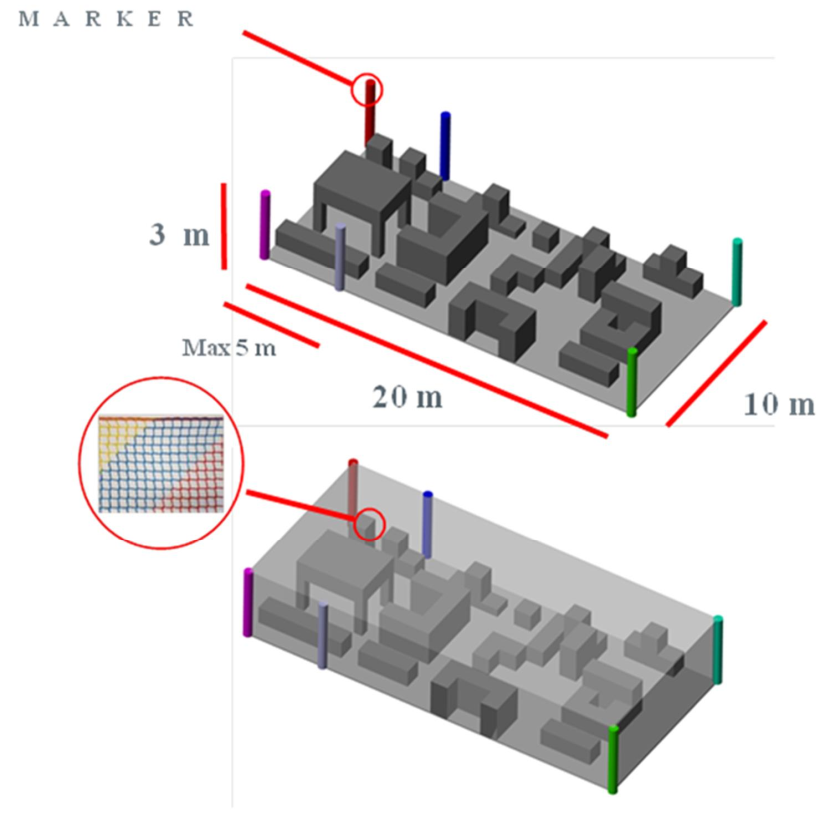
\includegraphics[width=0.6\textwidth]{Images/fig25-contest-env.png}
    \caption[Example of proposed environment]{Example of proposed environment for the Leonardo Drone Contest.}
    \label{fig:chapter0:contest-env}
\end{figure}

This work aims to shed some light on the importance of the usage of different landmarks in the environment, and how the implementation reacts on these different landmarks. Furthermore, it has the purpose to understand the importance of different implementation decisions included in the algorithm and how these decisions impacted on the results.
%\pagebreak
\section*{Road map}
The current work is divided in five chapters:
\begin{itemize}
    \item{\textbf{Chapter 2} introduces background information useful to completely understand the proposed implementation}
    \item{\textbf{Chapter 3} explains and comments the implementation in the context of the competition}
    \item{\textbf{Chapter 4} exposes the different experiments done in order to evaluate the implementation}
    \item{\textbf{Chapter 5} discusses over the results of the experiments and comments on possible future works and enhancements}
\end{itemize}

	\cleardoublepage
\chapter{Background}
\label{ch:chapter1}

\section{Robot Operating System}
\label{sec:chapter1:ros}
The \ac{ROS} \cite{ros-website} is an open source middleware that provides inter-process communication through a message passing mechanism. It is also a collection of libraries, tools and conventions with the aim of simplify the development of software for robots. In this sense, one of the main components of the framework are the nodes, which encapsulate processes and/or algorithms.

\subsection{Nodes}
\label{subsec:chapter1:ros:nodes}
Nodes are processes that perform a specific computation. In the system the nodes communicate between them using a publisher/subscriber infrastructure based on topics. A node subscribes to a particular topic, and it will receive messages from a publisher node. This way, a publisher node is hid to the subscriber, reducing the coupling between them. The advantage of this mechanism is that nodes can be developed separately once the message structure is defined, forcing developers to implement clear interfaces for communication by using a message \ac{IDL}. Moreover, this enables a modular and distributed development of the robotic system, while providing some fault tolerance and reduced code complexity.

\subsection{Topics}
\label{subsec:chapter1:ros:topics}
As mentioned before, communication between nodes is done via a publisher/subscriber architecture based on topics, which are named buses over which messages are exchanged. There can be several publishers (as well as subscribers) for a topic. A node that generates data publishes all its information in a specific topic bus, consequently this information is consumed by those nodes subscribed to that topic. The transport protocol used for exchanging messages is defined at runtime and can be of two types: TCPROS or UDPROS. The description of these protocols is beyond the scope of this document and the reader is invited to read the ROS documentation for detailed information.

\begin{figure}
    \centering
    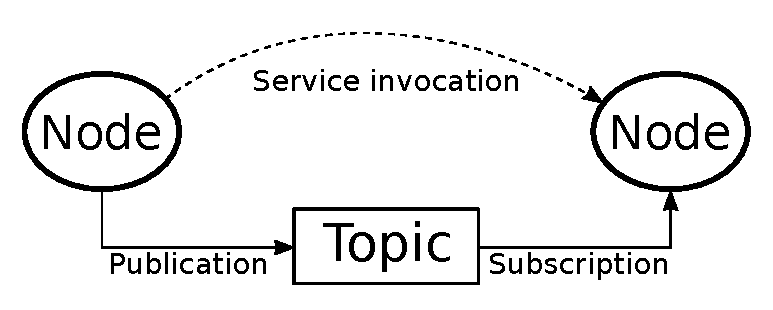
\includegraphics{Images/fig13-ros-basic-concept.eps}
    \caption[ROS basic concept]{ROS basic concepts. Two nodes communicate between them using the messages published in a topic. One node is responsible of publishing the topic, while the other subscribes and receives the messages of that particular topic. Furthermore, the node in the left calls a service provided by the node in the right, so that node will perform some computation and will return the result. \cite{ros-website}}
    \label{fig:chapter1:ros:basic_concepts}
\end{figure}

\subsection{Services}
\label{subsec:chapter1:ros:services}
As well as topics, services are a way to communicate nodes. The difference is that topics are an asynchronous way of communication, while services are synchronous. The key difference lies on the ability of nodes to decide when to trigger a service. Hence, services are used in between nodes to retrieve specific information or to request another node to carry out a computation beyond caller's node scope.


\subsection{Tools}
\label{subsec:chapter1:ros:tools}
Regarding the tools provided by ROS, one that is crucial for debugging and/or experimentation is the bag recording and playback. Since the exchange of messages between nodes is anonymous (meaning that nodes communicate between each others without knowing which node sent or received a message) it is possible to record the messages during a period of time, without taking into consideration which node sent a message and which node received it. This recorder bag is useful for debugging since it can be played back, hence reproducing a previous experiment. Also, it can be used for the development of new nodes that depend on the messages contained in the bag.\\

Another useful tool provided is \ac{RViz}, a 3D visualization tool. With this tool it is possible to see the robot, orientation, reference frames, covariance matrices, etc. In addition, it is possible to draw lines, arrows, text and others, onto the environment in order to see useful information that cannot be extracted from messages.

\subsection{MAVLink and MAVROS}
\label{sssec:chapter2:drone:mavlink}
%\nocite{mavlink}
MAVLink is a binary telemetry protocol designed for resource-constrained systems and bandwidth-constraint links, more specifically for drones of all kinds. As with ROS, it adopts a publisher-subscriber architecture, where data streams are published as topics. Its key features, as published in their website are:
\begin{itemize}
    \item Since its messages do not require any special framing, it is well suited for applications with very limited bandwidth.
    \item It provides methods for detecting package drops, corruption and for package authentication.
    \item Allows up to 255 concurrent systems on the network.
    \item Enables both offboard and onboard communications.
\end{itemize}
%\nocite{mavros}
MAVROS is the extension of MAVLink in ROS, with the additive of being a proxy for Ground Control Station tool. Its main features, as published in its website are:
\begin{itemize}
    \item Communication with autopilot via serial port, UDP or TCP .
    \item Internal proxy for Ground Control Station (serial, UDP, TCP).
    \item Plugin system for ROS-MAVLink translation.
    \item Parameter manipulation tool.
    \item Waypoint manipulation tool.
    \item PX4Flow support (by mavros\_extras).
    \item OFFBOARD mode support.
\end{itemize}

One characteristic that worth mentioning, is that it translates the \ac{NED} reference frames into \ac{ENU} reference frames, and vice-versa, so as to be compliant with ROS standard reference frames.

\subsection{RTAB-Map}
\label{subsec:chapter1:ros:octomap}
\ac{RTAB-Map} is a RGB-D, stereo and LiDAR graph-based \ac{SLAM} approach based on an incremental appearance-based loop closure detector. It allows to build a 3 dimensional map of the environment using a stereo camera, a LiDAR sensor and/or the odometry estimation. The map is built using a 3D occupancy grid by means of Octomap library, which builds a tree-based representation of the mapped area. Octomap library \enquote{performs a probabilistic occupancy estimation to ensure updatability and to cope with sensor noise}\cite{octomap-paper}.\\

The Octomap library generates an octotree, which is a hierarchical data structure used to generate spacial subdivision in 3 dimensions. Each node in an octotree represents a voxel, which is a cubic volume, which is at the same time, subdivided in eight smaller cubes until a given minimum voxel size called resolution. This way, the octotree data structure is used to build an occupancy grid of a volume. An example of a octotree can be seen in Figure~\ref{fig:chapter1:ros:octomap}, where the color of each occupied voxel represents its height: higher voxels are red-colored, while lower voxels are light-blue-colored.\\

\begin{figure}
    \centering
    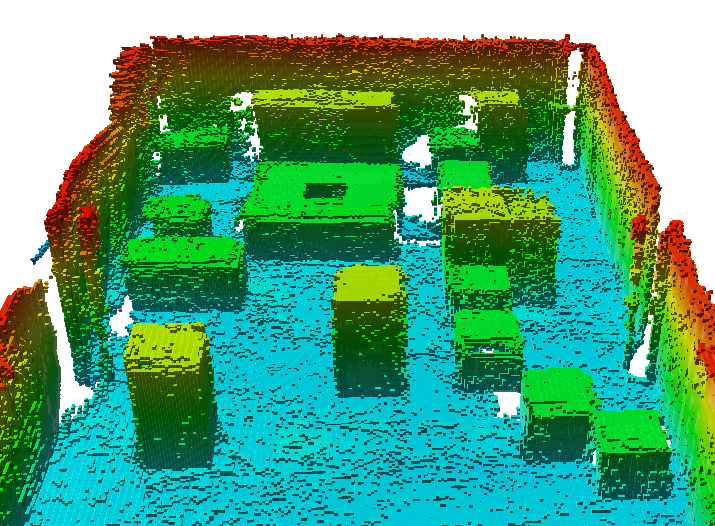
\includegraphics[width=\textwidth]{Images/fig14-octomap-colored2.png}
    \caption[Octomap example]{Octomap example. Octotree representation generated from data, showing occupied voxels only. \cite{octomap-paper}}
    \label{fig:chapter1:ros:octomap}
\end{figure}

RTAB-Map library, uses the Octomap library to store the 3D occupancy grid of the environment. The \inlinesrc{rtabmap_ros} node is the extension of the RTAB-Map library for ROS. It uses the information of the stereo camera or a RGB-D camera and/or a LiDAR information to create a cloud point that is used to build the map. Furthermore, it uses the provided odometry to estimate and correct the robot's pose into the 3D map. An example of this procedure can be seen in Figure~\ref{fig:chapter1:ros:rtabmap}.

\begin{figure}
    \centering
    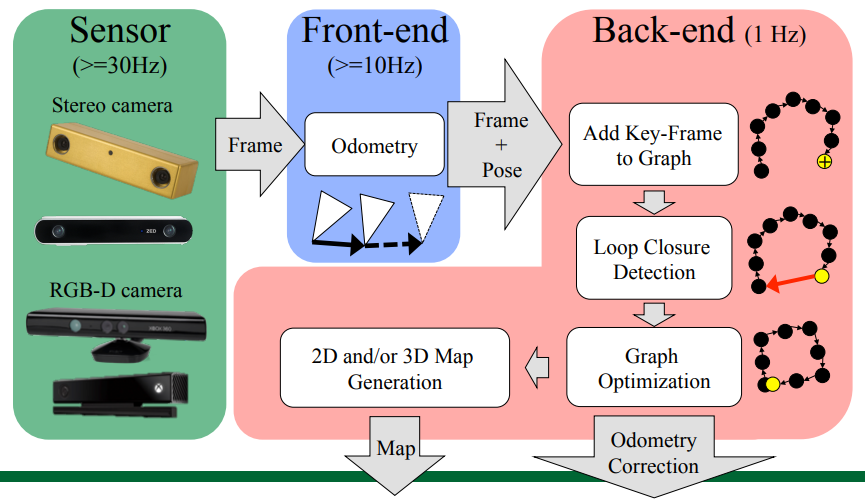
\includegraphics[width=\textwidth]{Images/fig14-rtabmap3.png}
    \caption[RTAB-Map example]{RTAB-Map example. An stereo camera or a RGB-D camera is used among the odometry estimation. Both are used to generate a 3D occupancy grid using Octomap library, and to correct the odometry estimation. \cite{rtabmap-presentation}}
    \label{fig:chapter1:ros:rtabmap}
\end{figure}

\section{Transformations}
\label{sec:chapter1:transform}
A robot, in this case the drone, can be considered as a rigid body that moves and rotates around the environment. Hence, it is necessary to model the drone displacement in space, and this can be done by decomposing the movement as translations and rotations.

\subsection{Translation}
\label{subsec:chapter1:transform:translation}
Given a vector $\bm{b} = \begin{bmatrix}b_x & b_y & b_z\end{bmatrix}^T$ that represents the center of mass of a rigid body, a translation that displaces $\bm{b}$ parallel to itself of a given vector $\bm{t}$ can be defined as:
\begin{align*}
    \bm{b} + \bm{t} = \begin{bmatrix}
        b_x \\ b_y \\ b_z
    \end{bmatrix} + \begin{bmatrix}
    t_1 \\ t_2 \\ t_3
\end{bmatrix} = \begin{bmatrix}
        b_x + t_1\\ b_y + t_2 \\ b_z + t_3
\end{bmatrix}
\end{align*}
Given a point $\mathcal{P}$ represented in the reference frame $\mathcal{R}_m$ by $\bm{v_P^m}$ will be represented in the reference frame $\mathcal{R}_n$ by:
\begin{align*}
    \bm{v_P^n} = \bm{v_P^m} + \bm{t_m^k}
\end{align*}

\subsection{Rotation}
\label{subsec:chapter1:transform:rotation}
In three dimensional space, any displacement of a rigid body is equivalent to a single rotation of a given angle about some axis that contains the point. It is possible to express the previous statement as $\bm{v} = \bm{u} * \theta$, being $\bm{u}$ a unit vector representing the axis and $\theta$ the angle.\\

Unlike with translations, two or more rotations cannot be simply the sum of the related vectors. A rotation can be described assuming a rigid body in a reference frame with its origin fixed, while the unit vectors are changed under the rotation. This way, a rotation is characterized by the mathematical relation of these two reference frames. Hence, in order to represent a rotation, two reference frames with a common origin are needed, as shown in Figure~\ref{fig:chapter1:transformation:rotation:3d-example}. At the beginning the two reference frames coincide, then one of them is rotated around the origin by an arbitrary angle. After this procedure, the two reference frames are not coincident anymore, however, both share the same origin.\\

\begin{figure}
    \centering
    \includegraphics[width=\textwidth]{Images/fig17-3D-rotation-example}
    \caption[Rotation around origin]{Rotation around origin. The reference frame at the left is rotated around Y axis and, as result, a new reference frame is obtained, both sharing the same origin.}
    \label{fig:chapter1:transformation:rotation:3d-example}
\end{figure}

The rotation by any angle of any axis can be represented in a matrix form, $\bm{R_n^m}$, where each column of the matrix represents the unit vector of $R_n$ in $R_m$, so it represents the rotated frame $R_n$ with respect the fixed frame $R_m$ with common origin. Furthermore, it is possible to show that matrix $\bm{R_n^m}$ is \emph{orthonormal}, which means that its inverse is equal to its transpose.\\

Given the matrix representation of a rotation, it is possible to provide a way to rotate a vector in the space. When the reference frames origins are the same, the rotation of a vector is possible by multiplying it by the rotation matrix around an axis: $\bm{v^m} = \bm{R_n^m} \bm{v^n}$. This kind of rotations are called \emph{elementary rotations}, and given that there are three axis in a 3D space, three different elementary rotations can be defined:
\begin{enumerate}
    \item{Rotation around axis $x$: \begin{align*}
            \bm{R_{x, \theta}} = \begin{bmatrix}
                1 & 0 & 0 \\ 0 & \cos{\left(\theta\right)} & -\sin{\left(\theta\right)} \\ 0 & \sin{\left(\theta\right)} & \cos{\left(\theta\right)}
            \end{bmatrix}
    \end{align*}}
    \item{Rotation around axis $y$: \begin{align*}
        \bm{R_{y, \theta}} = \begin{bmatrix}
             \cos{\left(\theta\right)} & 0 &  \sin{\left(\theta\right)} \\ 0 & 1 & 0 \\  -\sin{\left(\theta\right)} & 0 & \cos{\left(\theta\right)}
        \end{bmatrix}
    \end{align*}}
    \item{Rotation around axis $y$: \begin{align*}
        \bm{R_{z, \theta}} = \begin{bmatrix}
            \cos{\left(\theta\right)} & -\sin{\left(\theta\right)} & 0 \\ \sin{\left(\theta\right)} & \cos{\left(\theta\right)} & 0 \\ 0 & 0 & 1
        \end{bmatrix}
    \end{align*}}
\end{enumerate}

As mentioned, unlike translations, rotations cannot be summed. Hence, if two consecutive rotations need to be performed around two axis, a multiplication is needed:
\begin{align}
    \bm{R_{y,x}} = \bm{R_{x, \alpha}} * \bm{R_{y, \beta}}
\end{align}
where $\bm{R_{y,x}}$ is the rotation around axis $y$ by an angle $\beta$ followed by a rotation around the new axis $x$ by an angle $\alpha$, as shown in Figure~\ref{fig:chapter1:transform:rotation_z_x}.

\begin{figure}
    \centering
    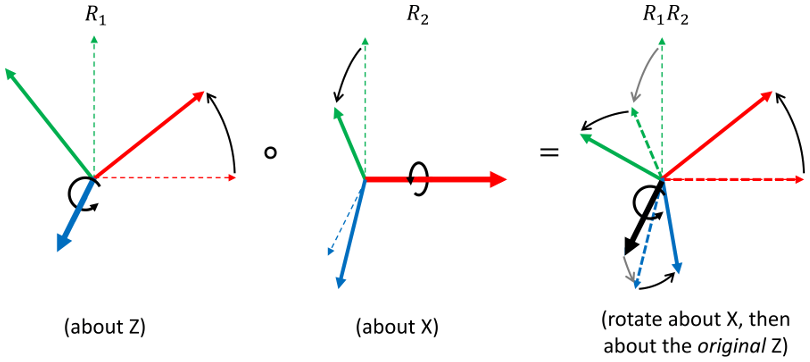
\includegraphics[width=\textwidth]{Images/fig16-rotations.png}
    \caption[Rotation around axis $z$ followed by rotation about axis $x$]{Rotation about axis $z$ followed by rotation about axis $x$. The second rotation is performed about the original axis $z$. This final rotation can be achieve by multiplying $R_1$ and $R_2$.\cite{hauser-robotics-systems}}
    \label{fig:chapter1:transform:rotation_z_x}
\end{figure}

\subsection{Homogeneous Transform}
\label{subsec:chapter1:transform:rototranslation}
A rotation and a translation can be accomplished as follow: $\hat{\bm{v}} = \bm{R}\bm{v} + \bm{t}$. Nevertheless, this can be achieve by using \emph{homogeneous coordinates}, where the point $\bm{v}$, expressed in its homogeneous representation, is $\bm{v} = \begin{bmatrix}v_x & v_y & v_z & 1\end{bmatrix}^T$. This way, the rotation and translation of a point can be accomplished by multiplying the 3D point with the homogeneous transformation matrix:
\begin{align}
    \bm{T}_m^n &= \begin{bmatrix}
        \bm{R}_m^n & \bm{t} \\
        \bm{0} & 1
    \end{bmatrix}
    \label{eq:chapter1:transform:homogeneous_transform}\\
    \hat{\bm{v}}^n &= \bm{T}_m^n\bm{v}^m
\end{align}
As can be noticed in equation~(\ref{eq:chapter1:transform:homogeneous_transform}), the homogeneous transformation is represented by a $4 \times 4$ matrix, and unlike the pure rotation matrix showed in Section~\ref{subsec:chapter1:transform:rotation}, the inverse of the homogeneous transformation is not equal to its transpose. The inverse of the homogeneous transformation is equivalent to:
\begin{align}
    \bm{T}^{-1} &= \begin{bmatrix}
        \bm{R}^T & -\bm{R}^T\bm{t} \\
        \bm{0} & 1
    \end{bmatrix}
\end{align}

\begin{figure}
    \centering
    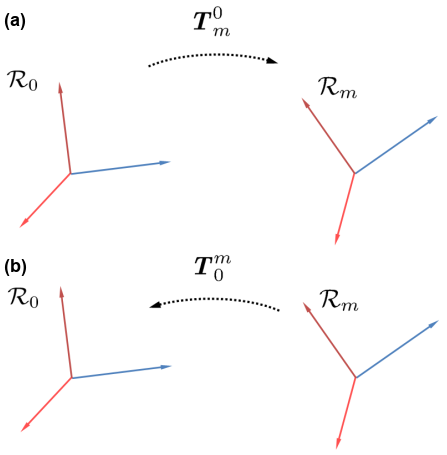
\includegraphics[width=0.5\textwidth]{Images/fig15-homogeneous-transform.png}
    \caption[Example of a Homogeneous transform]{Example of a Homogeneous transform. \textbf{(a)} Transformation $\bm{T}_m^0$ is applied to a point in reference frame $\mathcal{R}_0$ to express it in reference frame $\mathcal{R}_m$. \textbf{(b)} The inverse transformation is applied, so to express the point in reference frame $\mathcal{R}_m$ into reference frame $\mathcal{R}_0$.  \cite{bona-dynamic-modelling}}
    \label{fig:chapter1:transform:homogeneous}
\end{figure}

\section{Kalman Filter}
\label{sec:chapter1:kf}
%\nocite{intro-robotics}

Introduced by \cite{kalman}, the \ac{KF} provides a recursive method for estimating the state of a dynamic system with presence of noise. It is a technique for filtering and prediction in \emph{linear Gaussian systems} and applicable only to continuous states. One of its key features is that it simultaneously maintains estimates of the state vector and the estimate error covariance. It assures that the posteriors are Gaussian if the Markov assumption is hold, in addition to three conditions. The Markov assumption states that the past and future data are independent if one knows the current state; the other three conditions are the following:
\begin{enumerate}
    \item{The state transition probability $p\left( x_t | u_t, x_{t-1}\right)$ must be a linear function in its arguments. This is guaranteed by $ x_t = A_t x_{t-1} + B_t u_t + \epsilon_t $. Here, $x_t$ and $x_{t-1}$ are the state vectors, of size $n$, and $u_t$ represents the control vector, of size $m$, at time $t$; $A_t$ and $B_t$ are matrices of size $n \times n$ and $n\times m$ respectively. In this way, the state transition function becomes linear in its arguments, hence KF assumes a linear system dynamics. \\\\ $\epsilon_t$ represents the uncertainty introduced by the state transition, and it is a Gaussian random variable with zero mean and $R_t$ covariance.}
    \item{The measurement probability $p\left(z_t | x_t\right)$ must be linear in its arguments. This is guaranteed by $z_t = C_t x_t + \delta_t$, where $z_t$ represents the measurement vector of size $k$, $C_t$ is a matrix of size $k \times n$ and $\delta_t$ is a Gaussian noise with zero mean and $Q_t$ covariance.}
    \item{The initial belief should be normally distributed.}
\end{enumerate}
Given these three conditions, we are guaranteed that the posterior probability is Gaussian.

\begin{algorithm}[h]
    \caption{Kalman Filter algorithm}
    \label{alg:chapter1:kf}

    \BlankLine
    \KwIn{$\mu_{t-1}$, $\Sigma_{t-1}$, $u_t$, $z_t$}
    \BlankLine
    $\hat\mu_t = A_t \mu_{t-1} + B_t u_t$ \\
    $\hat\Sigma_t = A_t \Sigma_{t-1} A_t^T + R_t$ \\
    \BlankLine
    $K_t = \hat\Sigma_t C_t^T \left(C_t \hat\Sigma_t C_t^T + Q_t\right)^{-1}$ \\
    $\mu_t = \hat\mu_t + K_t \left(z_t - C_t \hat\mu_t \right) $ \\
    $\Sigma_t = (I - K_t C_t) \hat\Sigma_t$ \\
    \BlankLine
    \Return{$\mu_t$, $\Sigma_t$}
\end{algorithm}

The KF can be seen in Algorithm~\ref{alg:chapter1:kf} and its input is the belief at time $t-1$, represented by its mean ($\mu_{t-1}$) and its covariance ($\Sigma_{t-1}$), in addition to the control vector ($u_t$) and the observations ($z_t$). As a result, it returns the current belief characterized by its mean $\mu_t$ and covariance $\Sigma_t$. \\

The first step in the algorithm (lines 1 and 2), represent the prediction step. It calculates the current belief before incorporating the observations, but after adding the control vector. The estimated belief is characterized by its mean, $\hat\mu_t$ , and its covariance $\hat\Sigma_t$.\\

The second step (from line 3 to 5) starts by calculating $K_t$, the Kalman gain, which specifies the degree in which the observation is incorporated to the new state estimate. $K_t$ can be seen as the weighting factor that weights the relationship between the accuracy of the predicted state estimate and the observation noise. When $K_t$ is large, the observations have more importance in the final estimate; while if $K_t$ is small, the observations do not have much importance in the correction step. Following, at line 4, the new mean is estimated by means of the Kalman gain and the \emph{innovation}, which is the difference between the observation $z_t$ and the expected measurement $C_t \hat\mu_t$. Finally, the new covariance is calculated.

\subsection{Extended Kalman Filter}
\label{subsec:chapter1:kf:ekf}

The linearity conditions that make the KF to work are, in some cases, far from reality: state transition functions and measurements are rarely linear in practice. The \ac{EKF} works through a process of linearization, where nonlinear state transition and observation functions are approximated by a Taylor series expansion. \\

\begin{figure}
    \centering
    \includegraphics[width=\textwidth]{Images/fig1-kf-ekf.png}
    \caption[Linear and nonlinear transformation of a Gaussian random variable]{Linear \textbf{(a)} and nonlinear \textbf{(b)} transformation of a Gaussian random variable. The lower right plot shows the density function of the random variable. The upper right plot shows the transformation of the random variable. The upper left plot shows the resulting density function. \cite{prob-robotics}}
    \label{fig:chapter1:kf:ekf:cmp-kf-ekf}
\end{figure}

The Figure~\ref{fig:chapter1:kf:ekf:cmp-kf-ekf}a shows the linear transformation of a random Gaussian variable, whose density function is $\mathcal{N}\left(x; \mu, \sigma^2 \right)$. Assuming that the random variable is transformed using a linear function $y = ax + b$, the resulting random variable will be Gaussian with mean $a\mu + b$ and variance $a^2 \sigma^2$.\\

However, as shown in Figure~\ref{fig:chapter1:kf:ekf:cmp-kf-ekf}b, this does not happen if the transformation is not linear. In this case, assuming the original random variable is transformed using a nonlinear function $g$, the density of the resulting random variable is not Gaussian anymore.\\

The state transition probability and observation probabilities are ruled by nonlinear functions $g$ and $h$ respectively. Matrices $A$ and $B$ are replaced by function $g\left(u_t, x_{t-1}\right)$ and matrix $H$ is replaced by function $h \left(x_t\right)$, making the belief not Gaussian. This is solved in EKF by approximating to the true belief, not the exact one as happens with linear KF. The approximation is done using a linearization method that approximates the nonlinear function by a linear function that is tangent to it, thereby maintaining the Gaussian properties of the posterior belief. \\

The used method is the first order Taylor expansion, which constructs a linear approximation of a function $g$ from $g$'s value and slope, which is given by
\begin{equation}
    g' \left(u_t, x_{t-1}\right) = \frac{\partial g\left(u_t, x_{t-1}\right)}{\partial x_{t-1}}
    \label{eq:chapter1:kf:ekf:g-derivative}
\end{equation}

 Since $g$ depends on the control variable $u$ and the state $x$, we need to define a value for $x$, and the logical choice is the mean of the posterior in the previous time step: $\mu_{t-1}$. This way
 \begin{equation}
    g \left(u_t, x_{t-1}\right) = g \left(u_t, \mu_{t-1}\right) + g' \left(u_t, \mu_{t-1}\right)\left(x_{t-1} - \mu_{t-1}\right)
    \label{eq:chapter1:kf:ekf:g-mean-cov}
 \end{equation}
where $g'$ is the \emph{Jacobian} of $g$, usually expressed as $G_t$, and it depends on $u_t$ and $\mu_{t-1}$, hence it changes through time.\\

The same linearization is applied to the observation function $h$:
\begin{equation}
    h\left(x_t\right) = h\left(\hat\mu_t\right) + h'\left(\hat\mu_t\right)\left(x_t - \hat\mu_t\right)
\end{equation}
\begin{equation}
        h'\left(\hat\mu_t\right) = \frac{\partial h\left(x_t\right)}{\partial x_t}
\end{equation}
where $h'$ is the Jacobian of $h$, usually expressed as $H_t$. In this case, the linearization is done around $\hat\mu_t$, which is the state estimate just before computing $h$.\\

\begin{figure}[h]
    \centering
    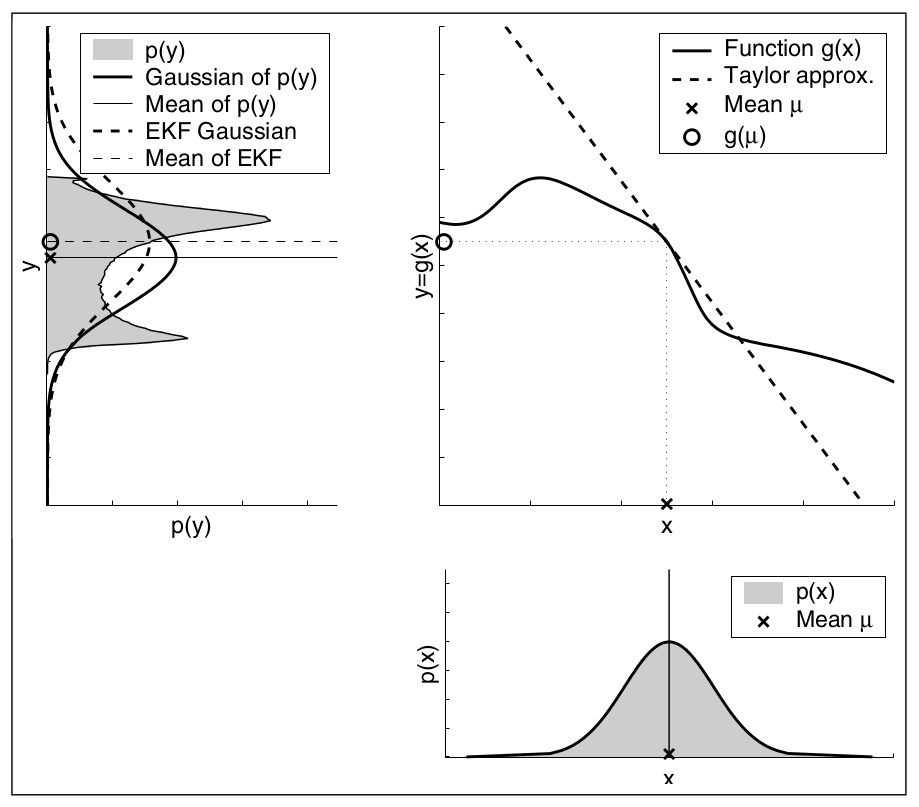
\includegraphics{Images/fig2-ekf-linearization.png}
    \caption[Linearization applied in EKF]{Linearization applied in EKF. In this case, the nonlinear function $g$ is approximated using first order Taylor expansion, that is a linear function tangent to $g$ at the mean of the original density function. The linearization is not perfect, so it adds an error, depicted in the upper left plot. This error is the difference between the dashed line and the solid line. \cite{prob-robotics}}
    \label{fig:chapter1:kf:ekf:ekf-linearization}
\end{figure}

The Figure~\ref{fig:chapter1:kf:ekf:ekf-linearization} depicts the approximation of $g$ by a linear function that is tangent around its mean. The resulting density function is shown in the upper left plot with a dashed line, that is similar to the original density function.\\

\begin{algorithm}[h]
    \caption{Extended Kalman Filter algorithm}
    \label{alg:chapter1:kf:ekf}

    \BlankLine
    \KwIn{$\mu_{t-1}$, $\Sigma_{t-1}$, $u_t$, $z_t$}
    \BlankLine
    $\hat\mu_t = g \left(u_t, \mu_{t-1}\right)$ \\
    $\hat\Sigma_t = G_t \Sigma_{t-1} G_t^T + R_t$ \\
    \BlankLine
    $K_t = \hat\Sigma_t H_t^T \left(H_t \hat\Sigma_t H_t^T + Q_t\right)^{-1}$ \\
    $\mu_t = \hat\mu_t + K_t \left(z_t - h \left(\hat\mu_t\right) \right) $ \\
    $\Sigma_t = (I - K_t H_t) \hat\Sigma_t$ \\
    \BlankLine
    \Return{$\mu_t$, $\Sigma_t$}
\end{algorithm}

The EKF algorithm can be seen in Algorithm~\ref{alg:chapter1:kf:ekf}, and it is similar to Algorithm~\ref{alg:chapter1:kf}. The difference lies in the usage of the nonlinear functions $g$ and $h$ and their Jacobians, $G_t$ and $H_t$ respectively.

\section{Simultaneous Localization and Mapping}
\label{sec:chapter1:slam}
Among all the problems faced by autonomous mobile robots, two of them are relevant for this work: localization and mapping. The former one, is related to the problem of where the robot is, while the later is related to building a map of the environment. However, in order to accurately localize itself the robot needs a map of the environment in which it is immersed in, and, in order to build a map, it needs to know where it currently is, giving us a chicken-egg situation. Hence, the \ac{SLAM} problem appears when the robot has no knowledge of its localization nor its environment map, while measurements and controls are given.\\

The problem of building a map can be summarized in the following steps:
\begin{enumerate}
    \item{The robot senses the environment using its sensors}
    \item{It creates a representation of the acquired data}
    \item{It integrates the processed sensor data with the previously learned map structure}
\end{enumerate}

While this process can be done by manually moving the robot around the environment, it is more challenging to build the map while the robot is moving autonomously. \\

%\nocite{intro-aut-mobile-robots}
On the other hand, assuming that the robot already knows the map, the localization problem could be trivial if no noise is present at all. The sensors, wheel encoders, different kinds of terrain, battery life, etc, all of these can make the robot to increase its uncertainty related to where it is. As robot moves around the environment it uses its sensors to estimate its position, increasing its uncertainty regarding its position relative to the map. At some point, the robot will "see" a known landmark or feature in the environment, correcting its position while reducing the uncertainty.\\
\begin{figure}
    \centering
    \includegraphics[width=\textwidth]{Images/fig3-slam.png}
    \caption[Example of SLAM problem]{At the beginning \textbf{(a)} the robot has low uncertainty regarding its pose. As it moves around the environment its uncertainty, represented by the dark gray ellipsis, grows \textbf{(b), (c), (d)}, until it sees a known landmark \textbf{(e)}, making the position uncertainty to shrink. \cite{intro-aut-mobile-robots}}
    \label{fig:chapter1:slam}
\end{figure}

The localization and mapping problems can be solved together by using a SLAM technique, with which the robot will build the map while localizing itself in it. An example of this problem can be seen in Figure~\ref{fig:chapter1:slam}, where a robot moves around the environment and sees some features or landmarks. The uncertainty regarding its position is low when it starts, and keeps growing while it moves around. At the end, it sees a known landmark ($m_0$) making the uncertainty to shrink. As can be seen in the figure, the robot adds new landmarks to the map ($m_1$ and $m_2$) with their corresponding uncertainty, and when the robot sees the first landmark, not only its own uncertainty decreases, but also the two new landmarks' uncertainty. In this way, the robot's position is correlated with the observations' position estimates.\\

The idea of the SLAM problem is to estimate a posterior belief that involves not only the robot pose, but also the map: $p\left(x_t, m | z_{1:t}, u_{1:t}\right)$, where $x_t$ is the robot's pose at time $t$, $m$ is the map, $z_{1:t}$ are the measurements, and $u_{1:t}$ are the controls given to the robot.

\subsection{EKF-SLAM}
\label{subsec:chapter1:slam:ekfslam}
The SLAM problem can be addressed, between others, using an EKF approach. The algorithm proceeds in the same way as shown in Section~\ref{subsec:chapter1:kf:ekf}, being $\mu$ a state vector containing the information for the robot pose ($q_r$) and the landmarks' pose ($m_i$):
\begin{equation}
    \mu = \begin{bmatrix}
        q_r & m_0 & \dots & m_{n-1}
    \end{bmatrix}^T
\end{equation}

One thing that is worth mentioning is that in EKF-SLAM maps are \emph{feature based}. This means that the features or landmarks are assumed to be points in the space: if the robot sees, for example, a chair, it will store a point that represents the chair in space. Also, as explained before, it assumes Gaussian noise for the robot motion and observations.\\

The EKF-SLAM algorithm estimates the robot's pose in addition to all encountered landmarks' poses along its way. Thus, there is a correspondence between robot's pose and landmarks, and that is why it is necessary to include the landmarks information into the state vector. Hence, the algorithm estimates the posterior $p\left(\mu_t | z_t, u_t\right)$.\\

\begin{algorithm}[h]
    \caption{EKF-SLAM algorithm}
    \label{alg:chapter1:slam:ekfslam}
    \BlankLine
    \KwIn{$\mu_{t-1}$, $\Sigma_{t-1}$, $u_t$, $z_t$}
    \BlankLine
    $\hat\mu_t = g\left(\mu_{t-1}, u_t\right)$\;
    $G_t = computeJacobian\left(g\right)$\;
    $\hat\Sigma_t = G_t \Sigma_{t-1} G_t^T + R_t$\;
    \BlankLine
    \ForEach{landmark observation $z_t^i$}{
        \BlankLine
        \If{landmark $i$ has not being seen before}{
            $addLandmarkToStateVector\left( z_t^i \right)$
        }
        \BlankLine
        $H_t^i = computeJacobian\left( h^i \right)$\;
        $v^i =  z_t^i - h^i \left( \hat\mu_t \right)$\;
        $S = H_t^i \hat\Sigma_t H_t^{iT} + Q_t$\;
        $K_t^i = \hat\Sigma_t H_t^{iT} S^{-1}$ \;
        $\mu_t = \hat\mu_t + K_t^i \left( v^i \right) $ \;
        $\Sigma_t = (I - K_t^i H_t^i) \hat\Sigma_t$ \;
    }
    \BlankLine
    \Return{$\mu_t$, $\Sigma_t$}
\end{algorithm}

Assuming the robot's pose is composed by $x$, $y$, $\theta$ , the markers' pose is composed by $x$, $y$, and there are $N$ markers, the state vector $\mu$ will have a length of $3 \times 2N$, and the covariance matrix $\Sigma$ will have a size of $(3 \times 2N) \times (3 \times 2N)$.\\

The algorithm can be seen in Algorithm~\ref{alg:chapter1:slam:ekfslam}. From lines 1 to 3, it computes the state vector and covariance matrix updates; the function $computeJacobian$ computes, indeed, the Jacobian matrix for the motion model $g$, and the resulting matrix has the same size as the covariance matrix and has the following characteristic:
\begin{align}
   G_t &= \begin{bmatrix}
        G_r & \textbf{0} \\
        \textbf{0} & \textbf{I}
    \end{bmatrix}\\
    G_r &= \begin{bmatrix}
    \frac{\partial x'}{\partial \mu_{t-1,x}} & \frac{\partial x'}{\partial \mu_{t-1,y}} & \frac{\partial x'}{\partial \mu_{t-1,\theta}}\\
    \frac{\partial y'}{\partial \mu_{t-1,x}} & \frac{\partial y'}{\partial \mu_{t-1,y}} & \frac{\partial y'}{\partial \mu_{t-1,\theta}}\\
    \frac{\partial \theta'}{\partial \mu_{t-1,x}} & \frac{\partial \theta'}{\partial \mu_{t-1,y}} & \frac{\partial \theta'}{\partial \mu_{t-1,\theta}}
\end{bmatrix}
\end{align}
where $\frac{\partial x'}{\partial \mu_{t-1,x}}$ is the derivative of $g$ along $x'$ dimension, taken with respect to $x$, $y$.. at $\mu_{t-1}$.\\

At line 4, it iterates through every observation $z_t$. At each time step $t$, a sensor obtains a set of observations $z^i$ of one of the $N$ landmarks. Each observation is associated with a map feature, and this association is accomplished by a prediction of the measurement that each feature would generate and a measure of the difference between the prediction and the sensor measurement. The prediction of the measurements can be obtained by the observation model $h^i$, which result is a vector of predicted features. If the observation $z^i$ comes from a landmark $i$, the following relation is hold:
\begin{align}
    z^i = h^i\left(x_t\right) + w^i
\end{align}
where $x_t$ is the true state and $w^i$ is the observation noise with covariance $Q_t$, and assumed to be zero mean, Gaussian, additive and independent of the process noise. If the landmark is not already in the state vector, at line 6 it is added by projecting the observation and calculating the landmark's pose, adding two new elements to the state vector and two new more columns and rows to the covariance matrix. At line 7 the Jacobian of the observation model is computed.\\

At line 8, the innovation is calculated while its covariance is calculated at line 9. The innovation measures the discrepancy between the predicted observation and the actual sensor measurement. At line 10 the Kalman gain is computed, and at line 11 the state vector is updated. The gain propagates the information through all the state vector, updating not only the robot's pose, but also the landmarks' poses.\\

The fact that the Kalman gain is not sparse is important, because observing a landmark not only improves the estimate of that landmark's pose, but also all the others, along with the robot's pose. This effect can be seen in Figure~\ref{fig:chapter1:slam}, with an additional explanation: most of the uncertainty of the landmarks' poses is caused by the robot's own uncertainty, so the location of those previously seen landmarks are correlated. When the robot gains information about its own pose, this information is propagated to the landmarks, and as result it improves the localization of other landmarks in the map.

\subsection{Adding new landmarks}
\label{subsec:chapter1:slam:ekfslam:addlandmarks}
So far, the existence and accuracy of a map was assumed. Nevertheless, this is not always true, and the construction of a map should somehow be done. Hopefully, EKF-SLAM algorithm considers the possibility of adding new landmarks to the map while doing the localization process with known landmarks. This process of adding new landmarks to the map is done via what is called inverse observation model, which handles the sensor measurements, identifies the new landmark, and adds it to the state vector.\\

The inverse observation model will produce the coordinates of the new landmark in the map, and this information will be added to the state vector, which will increase its size (in this case) by two new elements.
\begin{align}
    h^{-1}\left(\bm{x_r}, \bm{z}\right) &= \begin{bmatrix}
        x_l \\ y_l
    \end{bmatrix}
    \label{eq:chapter1:slam:ekfslam:inverseh}\\
    \bm{x_t} = y\left(\bm{x}, \bm{z}\right) &= \begin{bmatrix}
        \bm{x} \\ h^{-1}\left(\bm{x_r}, \bm{z}\right)
    \end{bmatrix}
    \label{eq:chapter1:slam:ekfslam:extension_y}
\end{align}
In equation~(\ref{eq:chapter1:slam:ekfslam:inverseh}) $\bm{x_r}$ refers to the elements in the state vector that corresponds to the robot's pose, and $\bm{z}$ refers to the observation elements, which can be, for example, range and bearing data. Since the state vector has a variable length, extending the covariance matrix is also needed whenever the robot sees a landmark that has not being seen previously. The extension of the covariance matrix is achieved as shown in equation~(\ref{eq:chapter1:slam:ekfslam:cov_update}).
\begin{align}
    \hat{\bm{\Sigma}} = \bm{Y_x} \bm{\Sigma} \bm{Y_x}^T + \bm{Y_z} \bm{Q}_t \bm{Y_z}^T
    \label{eq:chapter1:slam:ekfslam:cov_update}\\
    \bm{Y_x} = \frac{\partial y}{\partial x} = \begin{bmatrix}
        \frac{\partial x}{\partial x} \\ \frac{\partial h^{-1}}{\partial x}
    \end{bmatrix} = \begin{bmatrix}
    \bm{I} \\ \bm{G_x}
    \end{bmatrix}
    \label{eq:chapter1:slam:ekfslam:yx}\\
    \bm{Y_z} = \frac{\partial y}{\partial z} = \begin{bmatrix}
        \frac{\partial x}{\partial z} \\ \frac{\partial h^{-1}}{\partial z}
    \end{bmatrix} = \begin{bmatrix}
        \bm{0} \\ \bm{G_z}
    \end{bmatrix}
    \label{eq:chapter1:slam:ekfslam:yz}
\end{align}
where matrices $\bm{Gx}$ and $\bm{Gz}$ are the Jacobian of function $h^{-1}$ with respect to the state vector and the observation vector respectively. By substituting the Jacobians in equations (\ref{eq:chapter1:slam:ekfslam:yx}) and (\ref{eq:chapter1:slam:ekfslam:yz}) into equation~(\ref{eq:chapter1:slam:ekfslam:cov_update}), the following matrix is obtained:
\begin{align}
    \hat{\bm{\Sigma}} = \begin{bmatrix}
        \bm{\Sigma} & \bm{\Sigma} \bm{G_x}^T \\
        \bm{G_x} \bm{\Sigma} & \bm{G_x} \bm{\Sigma} \bm{G_x}^T + \bm{G_z} \bm{Q}_t \bm{G_z}^T
    \end{bmatrix}
    \label{eq:chapter1:slam:ekfslam:cov_update_full}
\end{align}\\

The linearized covariance update can be factored as shown in equation~(\ref{eq:chapter1:slam:ekfslam:factoring}) by assuming that $A \equiv 1$, $B \equiv 0$, $C \equiv 0$ and $D \equiv \bm{G_z}$
\begin{align}
    \begin{bmatrix}
        A & B \\ C & D
    \end{bmatrix} \begin{bmatrix}
        P & 0 \\ 0 & Q
    \end{bmatrix} \begin{bmatrix}
        A & B \\ C & D
    \end{bmatrix}^T &= \begin{bmatrix}
            APA^T + BQB^T & APC^T + BQD^T \\
            CPA^T + DQB^T & CPC^T + DQD^T
    \end{bmatrix}
    \label{eq:chapter1:slam:ekfslam:factoring}\\
    \hat{\bm{\Sigma}} &= \begin{bmatrix}
        \bm{1} & \bm{0} \\ \bm{G_x} & \bm{G_z}
    \end{bmatrix} \begin{bmatrix}
        \bm{\Sigma} & \bm{0} \\ \bm{0} & \bm{Q}_t
    \end{bmatrix} \begin{bmatrix}
        \bm{1} & \bm{0} \\ \bm{G_x} & \bm{G_z}
    \end{bmatrix}^T
    \label{eq:chapter1:slam:ekfslam:factored_cov_update}\\
\end{align}

\section{Normalized Estimation Error Squared}
\label{sec:chapter2:nees}
The Mahalanobis distance is a measure of the distance between a point and a distribution. It is a way to measure how many standard deviations is away the point from the mean of the distribution. The Mahalanobis distance of an observation $\bm{x} = \begin{bmatrix}x_1 & x_2 & \dots \end{bmatrix}$ with mean $\bm{\mu} = \begin{bmatrix}\mu_1 & \mu_2 & \dots \end{bmatrix}$, and covariance matrix $\Sigma$ is defined as:
\begin{equation}
    D = \sqrt{\left(\bm{x} - \bm{\mu}\right) \Sigma^{-1} \left(\bm{x} - \bm{\mu}\right)}
\end{equation}\\
Every time the drone observes a pole or a marker, a node responsible of identifying the landmark processes the features that distinguish it with respect to other landmarks, and publishes these features as a message. In the case of poles, the message type is \inlinesrc{RangeAndBearingPole}, which contains the range and bearing information, and in the case of markers the message type is \inlinesrc{Pose}, which contains the position and orientation information of the observed marker. Given this, each observation $z$ for a pole, is composed by three measurements, and each observation of a marker is composed by six measurements. After observing a landmark the Algorithm~(\ref{alg:chapter1:slam:ekfslam}) calculates the discrepancy between the observation $i$ and the predicted observation by the innovation ($v^i$), and its covariance ($S$), as
\begin{align*}
    v^i =  z_t^i - h^i \left( \hat\mu_t \right)\\
    S = H_t^i \hat\Sigma_t H_t^{iT} + Q_t
\end{align*}

The square of the Mahalanobis distance can be used in order to establish a correspondence between the observed measurements with the landmark features if the following is hold:
\begin{align}
    D_i^2 = v^i S^{-1} v^i < \chi_{d, 1-\alpha}^2
    \label{eq:chapter2:nees:innov_test}
\end{align}
where $d$ is the size of $h^i$ and $1-\alpha$ is the desired confidence level. This test is called individual compatibility, and when applied to the predicted state can be used to determine the subset of observation features that are compatible with the observation.\\

Furthermore, a state estimate is consistent if its state estimation error $\bm{x} - \hat{\bm{x}}$ satisfies
\begin{align*}
    \mathbb{E}\left[\bm{x} - \hat{\bm{x}}\right] = 0\\
    \mathbb{E}\left[\left(\bm{x} - \hat{\bm{x}}\right)\left(\bm{x} - \hat{\bm{x}}\right)^T\right] \le \Sigma
\end{align*}
When the ground truth $\bm{x}$ is available, a \ac{NEES} can be performed to check the consistency of the filter. NEES test can be defined as the squared Mahalanobis distance for the difference between $\bm{x}$ and $\hat{\bm{x}}$, and consistency can be checked with a $\chi^2$ test
\begin{align*}
    NEES = \left(\bm{x} - \hat{\bm{x}}\right) \Sigma^{-1} \left(\bm{x} - \hat{\bm{x}}\right) \le \chi_{d, 1-\alpha}^2
\end{align*}

However, the ground truth is only available in simulated environments thus, the consistency of the filter is maintained by using observations that satisfy the test in equation~(\ref{eq:chapter2:nees:innov_test}). This way, the filter will discard observations that do not satisfy the innovation test, maintaining a consistent estimation of the state and therefore, the map.

	\chapter{EKF-SLAM Implementation}
\label{ch:chapter2}
In Chapter~\ref{ch:chapter1} the EKF-SLAM algorithm in the context of SLAM was explained. As mentioned in Section~\ref{sec:chapter1:kf}, the algorithm can be summarized in two steps: prediction and correction. In the first stage involves the prediction of the next state of the system, meanwhile, during the correction stage, this estimation is updated. \\

In this chapter, an EKF-SLAM implementation is shown, starting from the used drone characteristics, going through the prediction and correction steps, and ending with the overall system's architecture.

\section{The Drone}
\label{sec:chapter2:drone}
\subsection{Characteristics}
\label{subsec:chapter2:drone:characteristics}
The drone considered for this analysis has a common characteristics, such as four rotors disposed as an X. The drone frame is called 3DR Iris Quadrotor, and can be seen in Figure~\ref{fig:chapter2:drone:frame}. Its total weight is XX kg., and it diameter is XX cm.\\

\begin{figure}
    \centering
    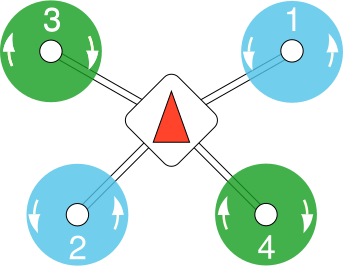
\includegraphics[width=0.5\textwidth]{Images/fig4-quad-frame.png}
    \caption{3DR Iris Quadrotor frame.}
    \label{fig:chapter2:drone:frame}
\end{figure}

\subsubsection{Flight Controller}
The flight controller used in this case is a PixHawk 4, and its characteristics are shown in Table~\ref{tab:chapter2:drone:px4fc}. It is worth mentioning that it includes an integrated accelerometer, a gyroscope, a magnetometer and a barometer.

\begin{table}
    \centering
    \begin{tabular}{cp{27em}}
        \toprule \textsc{Item} & \textsc{Description}\\
        \midrule
        \multirow{2}{*}{Main FMU processor} & STM32F765 \\
        & 32 Bit Arm® Cortex®-M7, 216MHz, 2MB memory, 512KB RAM \\
        \midrule
        \multirow{2}{*}{IO Processor} & STM32F100 \\
        & 32 Bit Arm® Cortex®-M3, 24MHz, 8KB SRAM \\
        \midrule
        \multirow{4}{*}{On-board sensors} & Accel/Gyro: ICM-20689 \\
        & Accel/Gyro: BMI055 \\
        & Magnetometer: IST8310 \\
        & Barometer: MS5611 \\
        \midrule
        GPS & ublox Neo-M8N GPS/GLONASS receiver; integrated magnetometer IST8310 \\
        \midrule
        \multirow{10}{*}{Interfaces} & 8-16 PWM outputs (8 from IO, 8 from FMU) \\
        & 3 dedicated PWM/Capture inputs on FMU \\
        & Dedicated R/C input for CPPM \\
        & Dedicated R/C input for Spektrum / DSM and S.Bus with analog / PWM RSSI input \\
        & Dedicated S.Bus servo output \\
        & 5 general purpose serial ports \\
        & 3 I2C ports \\
        & 4 SPI buses \\
        & Up to 2 CANBuses for dual CAN with serial ESC \\
        & Analog inputs for voltage / current of 2 batteries \\
        \midrule
        \multirow{3}{*}{Power System} & Power module output: 4.9~5.5V \\
        & USB Power Input: 4.75~5.25V \\
        & Servo Rail Input: 0~36V \\
        \midrule
        \multirow{2}{*}{Weight and Dimensions} & Weight: 15.8g \\
        & Dimensions: 44x84x12mm \\
        \midrule
        Operating temperature & -40 to 85°c \\
        \bottomrule
    \end{tabular}
    \caption[PixHawk 4 Specification]{Technical specification of the PixHawk 4 flight controller.}
    \label{tab:chapter2:drone:px4fc}
\end{table}

\subsubsection{Additional Sensors}
The drone was equipped with several sensors that are the input for localization, mapping and path planning algorithms, among others.\\

The localization and mapping algorithm makes use, in an indirect way, of monocular and stereo cameras, and laser range sensors. Four cameras were mounted in order to be able to have 360 range view, with cameras mounted every 90 degrees. Furthermore, two stereo cameras were mounted, one points forward in order to update the Octomap and the other points downwards in order to see the markers; Also, both of them are used to build a 3-dimensional map, used for obstacle avoidance and with the height estimation algorithm. Furthermore, eight laser range sensors were mounted every 45 degrees, and one laser range sensor was mounted pointing downwards in order to estimate the current drone height.

\subsection{Reference Frames}
\label{subsec:chapter2:drone:frames}
This system is composed by three reference frames linked with each other, as represented in Figure~\ref{fig:chapter2:drone:frames:frames}: \emph{map}, \emph{odom} and \emph{base\_link}. The \emph{map} frame, also called \emph{world} or \emph{global} frame, is the static reference frame, where the global drone's position and global markers' position is set. The odom reference frame is similar to the map frame, but the difference is that this frame drifts with time, as happens with the pure odometry. Finally, the base\_link frame, also referred as \emph{body} or \emph{local} frame, refers to the center of mass of the drone.\\

As mentioned before, all transformations within these reference frames are published by different nodes: the map to odom transformation is handled by the \emph{rtabmap} node, the odom to base\_link is handled by \emph{mavros} node. There are many other transformations in the system, but they are mainly related to the base\_link reference frame and the different cameras and sensors in the drone. \\
\begin{figure}
    \centering
    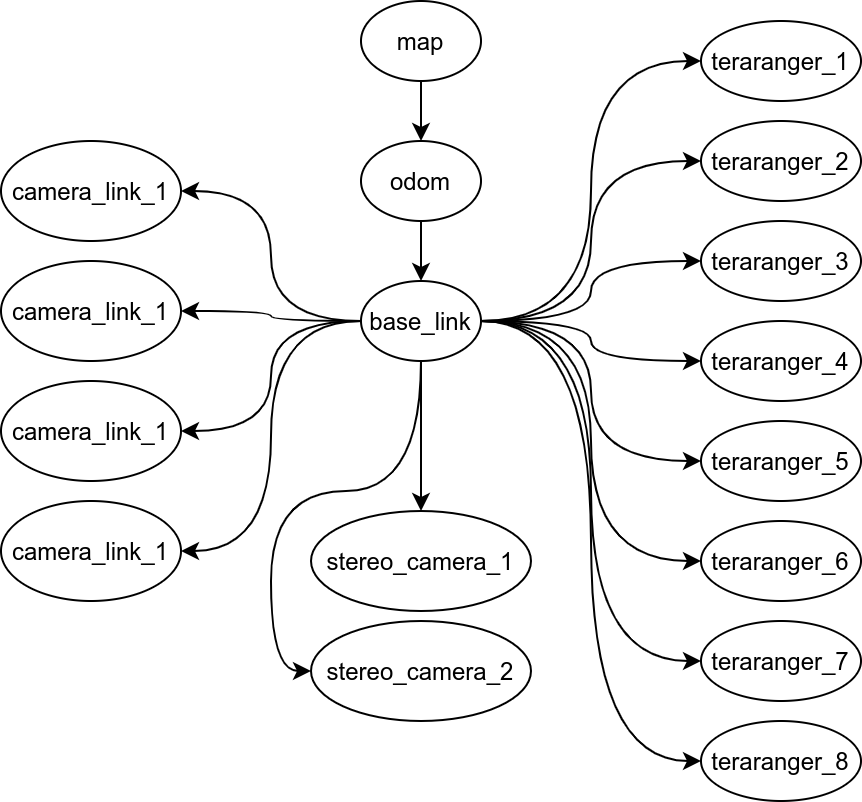
\includegraphics[width=0.5\textwidth]{Images/fig5-frames.png}
    \caption{Main reference frames in the system.}
    \label{fig:chapter2:drone:frames:frames}
\end{figure}

Finally, there is a transformation that worth mentioning: the \ac{NED} to \ac{ENU}. As mentioned in Section~\ref{sec:chapter1:ros}, ROS uses the ENU convention, while the convention adopted by the Aerospace community is the NED. Also, as mentioned in Section~\ref{sssec:chapter2:drone:mavlink}, MAVROS is in charge of doing and publish this transformation. In Figure~\ref{fig:chapter2:drone:frames:enu2ned} a simple scheme of the transformation can be seen. As explained before, this transform consists on rotating the X-axis and the Y-axis by 90 degrees, hence the homogeneous rotation matrix will have the following form:
\begin{align}
    R_{ENU}^{NED} & = \begin{bmatrix}
        0 & -1 & 0 & 0 \\
        0 & 0 & 1 & 0 \\
        -1 & 0 & 0 & 0 \\
        0 & 0 & 0 & 1
    \end{bmatrix}
\end{align}


\begin{figure}
    \centering
    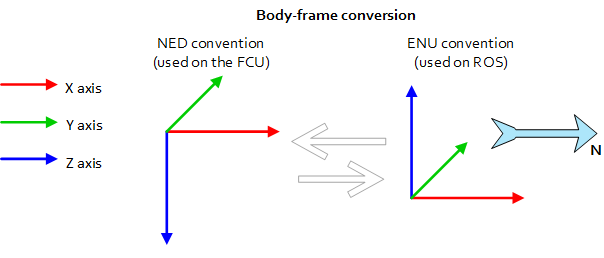
\includegraphics[width=\textwidth]{Images/fig6-ned2enu.png}
    \caption{NED to ENU conversion scheme. \cite{mavros}}
    \label{fig:chapter2:drone:frames:enu2ned}
\end{figure}

\section{Motion Model}
\label{sec:chapter2:prediction}
During the prediction step, the motion model and the covariance matrix update are computed. The motion model will update the state vector, which will store the position X, Y and Z in the global reference frame, and the orientation in the Z-axis of the drone. Fortunately MAVROS provides a node that makes odometry estimation based on different sensors outputs. The messages published by the odometry node, of type \inlinesrc{Odometry}, provide the linear velocity, the angular velocity and pose information. The velocity information is used to estimate the position in X, Y and Z, and the drone's orientation along the Z-axis. However, the velocity estimation provided by MAVROS is relative to the body reference frame, and this has to be transformed into the world reference frame, so before estimating the global position of the drone it is mandatory to do this transformation.

\begin{align}
    u &= \begin{bmatrix} v_x^b & v_y^b & v_z^b & \omega_x^b & \omega_y^b & \omega_z^b & \phi^b & \theta^b & \psi^b \end{bmatrix}^T\\
    v^w &= \textbf{T} * \begin{bmatrix} v_x^b \\ v_y^b \\ v_z^b \end{bmatrix}
\end{align}
where the control vector $u$ is composed by the linear velocities in the body reference frame ($v_x^b$, $v_y^b$, $v_z^b$), the angular velocities in the body reference frame ($\omega_x^b$, $\omega_y^b$, $\omega_z^b$) and the drone's orientation ($\phi^b$, $\theta^b$, $\psi^b$). Additionally, $\textbf{T}$ is the homogeneous transform (see Section~\ref{sec:chapter1:transform}) using the current orientation of the drone: $\phi^b$, $\theta^b$ and $\mu_{\psi}$. Notice the third element of the orientation ($\mu_{\psi}$), this is because the orientation over the Z-axis is estimated by the filter. As result, $v^w$ will be a column vector with the linear velocities in the global reference frame. \\

Given this, the motion model update can be summarized in the following calculation:
\begin{align}
    \hat\mu &=
    \begin{bmatrix}
        \mu_{t-1, x^w} \\ \mu_{t-1, y^w} \\ \mu_{t-1, z^w}
    \end{bmatrix}
    + \Delta t * v^w \\
    \hat\mu_{\psi} &= \mu_{t-1, \psi} + \Delta t * \omega_z^b
\end{align}

Then, $\textbf{G}_t$, which is the Jacobian matrix of the motion model, should be computed. As mentioned in Section~\ref{subsec:chapter1:slam:ekfslam}, it has the following characteristic:
\begin{align}
    G_t &= \begin{bmatrix}
        G_r & \textbf{0} \\
        \textbf{0} & \textbf{I}
    \end{bmatrix}\\
    G_r &= \begin{bmatrix}
        1 & 0 & 0 & G_{r, 14} \\
        0 & 1 & 0 & G_{r, 24} \\
        0 & 0 & 1 & 0 \\
        0 & 0 & 0 & 1
    \end{bmatrix}
\end{align}
\begin{align*}
     G_{r, 14} &= -\Delta t * (v_y^w * (c_{\phi} * c_{\psi} + s_{\theta} * s_{\phi} * s_{\psi}) - v_z^w * (c_{\psi} * s_{\phi} - c_{\phi} * s_{\theta} * s_{\psi}) + v_x^w * c_{\theta} * s_{\psi}) \\
     G_{r, 24} &= -\Delta t * (v_z^w * (c_{\psi} * s_{\phi} + c_{\phi} * s_{\theta} * c_{\psi}) -v_y^w * (c_{\phi} * s_{\psi} - s_{\theta} * s_{\phi} * c_{\psi}) + v_x^w * c_{\theta} * s_{\psi})
\end{align*}
where
\begin{alignat*}{3}
    c_{\phi} &= \cos{\left(u_{\phi}\right)}, \quad & c_{\theta} &= \cos{\left(u_{\theta}\right)}, \quad & c_{\psi} &= \cos{\left(\mu_{\psi}\right)} \\
    s_{\phi} &= \sin{\left(u_{\phi}\right)}, \quad & s_{\theta} &= \sin{\left(u_{\theta}\right)}, \quad & s_{\psi} &= \sin{\left(\mu_{\psi}\right)}
\end{alignat*}\\
The function $g$ that models the motion of the drone is assumed to be perfect and therefore noise free. So, before computing the covariance update, it is necessary to compute the process noise covariance matrix ($R_t$) that encodes the motion model noise which, in this case, is related to the underlying dynamics of the drone flight. The noise is assumed to be additive and Gaussian, and therefore, the motion model can be decomposed as:
\begin{equation}
    x_t = g(u_t, x_{t-1}) + \mathcal{N}\left(0, R_t\right)
    \label{eq:chapter2:prediction:motion_w_noise}
\end{equation}
\begin{equation}
    R_t = N * U * N^t
    \label{eq:chapter2:prediction:control_cov}
\end{equation}
the noise part in equation (\ref{eq:chapter2:prediction:motion_w_noise}) relates to the acceleration component that is, in this case, unknown. However, it is known from a theoretical perspective: the acceleration component in an accelerated movement is $\frac{1}{2}\Delta t^2 a$, where $a$ is the body's acceleration. Given this, we can assume that the noise component in the motion model is:
\begin{equation}
    \mathcal{N}\left(0, R_t\right) = \frac{1}{2} \Delta t^2 T_w^b \begin{bmatrix}
        a_x \\ a_y \\ a_z \\ a_{\psi}
    \end{bmatrix}
\end{equation}
where $T_w^b$ is the transformation matrix from body to world reference frame. The covariance of the process noise ($R_t$) can be decompose as shown in equation~(\ref{eq:chapter2:prediction:control_cov}), where matrix $N$ is the Jacobian of acceleration term  with respect to the state vector, and matrix $U$ is the estimated average acceleration.
\begin{equation}
    N = \frac{\partial \frac{1}{2} \Delta t^2 T_w^b \textbf{a}}{\partial \mu}
\end{equation}
\begin{equation}
    U = \textbf{I} * \begin{bmatrix}
        a_{avg, x} \\ a_{avg, y} \\ a_{avg, z} \\ a_{avg, \psi}
    \end{bmatrix}
\end{equation}
The multiplication in (\ref{eq:chapter2:prediction:control_cov}) provides an approximate mapping between the motion noise in control space and the motion noise in the state space.\\

Finally, the covariance update should be computed as follow
\begin{align}
    \hat\Sigma &= G_t * \Sigma * G_t^T + R_t
\end{align}

\section{Observation Models}
\label{sec:chapter2:correction}
While the drone is moving around the environment it senses different landmarks that may be included or not in the state vector. These observations will eventually improve the localization of the drone, and will improve the landmarks' poses if needed. The whole process involves the computation of the Jacobian of the observation model for the seen landmark, the computation of the Kalman gain, and the update of the state vector and covariance matrix.\\

To perform the correction step, EKF-SLAM needs a linearized observation model with additive Gaussian noise. In the case studied in this work, there are two kinds of landmarks and, therefore, two different observation models. The main difference between these two type of landmarks, is that the position of poles type is known, while it is not known in the case of markers. Hence, every time the robot "sees" a pole, the algorithm will update the drone's pose and the known markers' pose; while every time it "sees" a marker two course of action are possible:
\begin{enumerate}[a)]
    \item{if the marker is not known, it is added to the state vector, enlarging it along with the covariance matrix.}
    \item{if the marker is known, its pose, the pose of all other markers, and the drone's pose are updated.}
\end{enumerate}

The observation model is, as with the motion model in equation~(\ref{eq:chapter2:prediction:motion_w_noise}), assumed to be perfect and with an additive Gaussian noise. The noise here is related to the observation process, and so, related to the used sensors.
\begin{equation}
    z_i = h_i\left(x_t\right) + \mathcal{N}\left(0, Q_t\right)
    \label{eq:chapter2:correction:obs_w_noise}
\end{equation}
Consequently, the noise covariance matrix of the observation model cannot be deducted as with the noise covariance matrix of the motion model. In this case, the matrix should be constructed empirically based on the sensors' characteristics, and it has the following characteristic:
\begin{equation}
    Q_t = \begin{bmatrix}
        \sigma_1^2 &  & \textbf{0} \\
         & \ddots & \\
        \textbf{0} & & \sigma_n^2 \\
    \end{bmatrix}
\end{equation}\\
where the diagonal elements $\sigma_{1..n}$ are the standard deviation of the sensor. Depending on the sensor used, the diagonal elements can be the standard deviation for the range and bearing components (distance, azimuth and elevation), or others.\\

As shown in Algorithm~\ref{alg:chapter1:slam:ekfslam} several steps are followed during the correction part of the algorithm. After computing the observation model and its Jacobian matrix, the Kalman gain and the innovation should be calculated, and finally, the state vector and covariance matrix updates should be done.

\subsection{Observation model for Poles}
\label{subsec:chapter2:correction:poles}
In the case of Poles, a range and bearing method is used. In this case, since the poles have a known position, their information is not kept in the state vector and therefore, this information will be used for localization purposes.\\

A ROS node will publish the range and bearing information every time the drone sees a pole, and this information will be used to calculate the innovation based on the predicted range and bearing. Hence, the observation model used for poles is computed in the following way:
\begin{equation}
    \begin{bmatrix}
        p_{i, x}^b \\ p_{i, y}^b \\ p_{i, z}^b
    \end{bmatrix} = \bm{T_r}^{-1} \begin{bmatrix}
        p_{i, x}^w \\ p_{i, y}^w \\ p_{i, z}^w
\end{bmatrix}
\label{eq:chapter2:correction:pole:world2body_transform}
\end{equation}
\begin{equation}
    h_i(\hat\mu_t) = \begin{bmatrix}
        p_{i, \rho} \\ p_{i, \alpha} \\ p_{i, \beta}
    \end{bmatrix} = \begin{bmatrix}
    \sqrt{ p_{j, x^b}^2 + p_{j, y^b}^2 } \\
    \atantwo{p_{j, y}^b}{p_{j, x}^b} \\
    \atantwo{p_{j, z}^b}{p_{j,\rho}^b}
\end{bmatrix}
\label{eq:chapter2:correction:pole:range_bearing}
\end{equation}

In equation~(\ref{eq:chapter2:correction:pole:world2body_transform}), $\bm{T_r}^{-1}$ corresponds to the inverse of the homogeneous transformation matrix with respect to the current drone's pose, and elements $p_i^w$ are the $x$, $y$ and $z$ coordinates of the $i$ pole's tip in the world reference frame. This way, the global position of the pole $i$ is projected to the body reference frame. After that, the range ($\rho$), azimuth angle ($\alpha$) and elevation angle ($\beta$) are calculated, as shown in equation~(\ref{eq:chapter2:correction:pole:range_bearing}). In Figure~\ref{fig:chapter2:correction:poles:range_bearing} an example of the range and bearing is shown.
\begin{figure}[h]
    \centering
    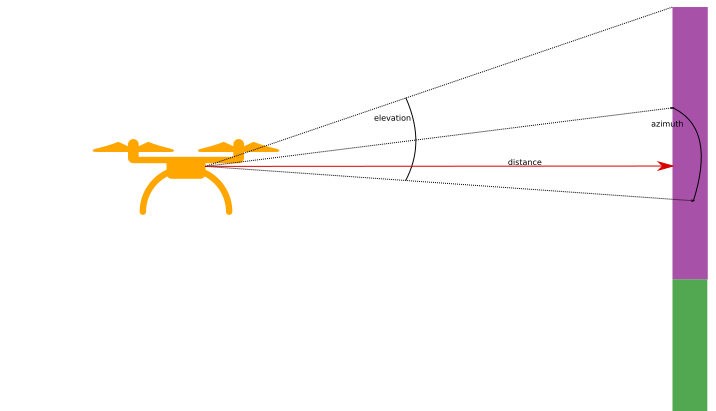
\includegraphics[width=\textwidth]{Images/fig7-range_and_bearing}
    \caption[Range and Bearing example]{Range and bearing example. The drone observes a pole, process the data from the sensors and estimates the distance ($\rho$), the elevation angle ($\beta$), and the azimuth angle ($\alpha$). The elevation angle is calculated based on the top extreme of the pole.}
    \label{fig:chapter2:correction:poles:range_bearing}
\end{figure}

Observing a pole affects only the drone's pose, and therefore, the Jacobian matrix of the observation model will have the following form:
\begin{equation}
    H_i = \begin{bmatrix}
        \frac{\partial \rho'}{\partial \mu_x} & \frac{\partial \rho'}{\partial \mu_y} & \frac{\partial \rho'}{\partial \mu_z} & \frac{\partial \rho'}{\partial \mu_{\psi}} & \dots & 0 \\
        \frac{\partial \alpha'}{\partial \mu_x} & \frac{\partial \alpha'}{\partial \mu_y} & \frac{\partial \alpha'}{\partial \mu_z} & \frac{\partial \alpha'}{\partial \mu_{\psi}} & \dots & 0 \\
        \frac{\partial \beta'}{\partial \mu_x} & \frac{\partial \beta'}{\partial \mu_y} & \frac{\partial \beta'}{\partial \mu_z} & \frac{\partial \beta'}{\partial \mu_{\psi}} & \dots & 0
    \end{bmatrix}
\end{equation}
where $\rho'$ corresponds to the distance part of the observation model, $\alpha'$ is the azimuth part, and $ \beta'$ the elevation part. The elements after the \nth{4} column are all 0, which means, as said before, that the observation of a pole will not affect the pose of the markers.

\subsection{Observation model for Markers}
\label{subsec:chapter2:correction:markers}

The observation model for the markers is a bit different. In this case a ROS node is responsible of detecting, tracking and publishing the pose of the markers with respect to the camera that has seen it. The ROS package responsible of this process is called \inlinesrc{visp_auto_tracker}, and publishes messages of type \inlinesrc{PoseStamped}, which provides the position and orientation of the seen marker. An example of this situation can be seen in Figure~\ref{fig:chapter2:correction:markers:example}.\\

\begin{figure}
    \centering
    \includegraphics[width=\textwidth]{Images/fig8-marker_example}
    \caption[Example of the drone observing a marker]{Example of the drone observing a marker. The camera visualize a marker and the node \inlinesrc{visp_auto_tracker} estimates its pose with respect to the camera reference frame.}
    \label{fig:chapter2:correction:markers:example}
\end{figure}

Every time the camera that points down sees a known marker, the \inlinesrc{visp_auto_tracker} node will publish the pose of that marker. This published pose is with respect to the camera which is not positioned at the drone's center of mass and so, a different transformation is needed. This process can be seen in equation~(\ref{eq:chapter2:correction:markers:world2body_trasnform}), in which the transformation of the marker's pose in the world reference frame is transformed to the pose in the camera reference frame.
\begin{equation}
    \begin{bmatrix}
        m_{i, x}^c \\ m_{i, y}^c \\ m_{i, z}^c \\ m_{i, \phi}^c \\ m_{i, \theta}^c \\ m_{i, \psi}^c
    \end{bmatrix} = (\bm{T_r} * \bm{T_c})^{-1} * \bm{T_m}
    \label{eq:chapter2:correction:markers:world2body_trasnform}
\end{equation}
where, $\bm{T_r}$ is the homogeneous transformation matrix of the drone's pose, $\bm{T_c}$ is the homogeneous transformation matrix of the camera's pose, and $\bm{T_m}$ is the homogeneous transformation of the marker's pose. The result is a vector that contains the marker's pose in the camera reference frame.\\

As mentioned before, observing a marker will update the drone's pose and that marker's pose, and therefore the Jacobian matrix of the observation model will have a different aspect from the pole's case. Here, the Jacobian can be split in two parts as shown in equation~(\ref{eq:chater2:correction:markers:jacobian}), where the left part, as with the poles, affects the drone's pose, while the right part of the matrix affects the seen marker's pose.
\begin{align}
    H_i &= \begin{bmatrix}
        \frac{\partial h_i(\hat\mu)}{\partial \mu_r} & \dots0\dots & \frac{\partial h_i(\hat\mu)}{\partial \mu_{m_i}} & \dots0\dots
    \end{bmatrix}
    \label{eq:chater2:correction:markers:jacobian}
\end{align}

The Jacobian matrices of the observation model with respect to the drone state and with respect the marker pose can be seen in Appendix~\ref{appendix:a}. It is worth to mention that the reason why this matrix only contains two sections different to zero is because of the relations between markers: observing a marker does not affect the pose of others, and therefore, the Jacobians of the observation model for marker $i$ with respect to marker $i+1$ or any other marker is 0.\\

Furthermore, unlike the case of poles, the markers' pose is unknown the first time, and therefore the algorithm will introduce their pose into the state vector when the drone sees a previously unknown marker.

\subsubsection{Adding new Markers}
\label{subsubsec:chapter2:correction:markers:add}
\nocite{slam-auto-mob-robots}
As mentioned in Section~\ref{subsec:chapter1:slam:ekfslam:addlandmarks}, to add new landmarks to the state vector an inverse observation model is needed. In the current case, the inverse observation model will project the observed marker's pose from the camera reference frame to the world reference frame. Equation~\ref{eq:chapter2:correction:markers:inverseh} shows the inverse observation model for markers where, similarly to the observation model, a set of transformations are performed but, this time, in order to obtain the pose of the seen marker in the world reference frame:
\begin{align}
    \begin{bmatrix}
        m_{i, x}^w \\ m_{i, y}^w \\ m_{i, z}^w \\ m_{i, \phi}^w \\ m_{i, \theta}^w \\ m_{i, \psi}^w
    \end{bmatrix} &= \bm{T_r} * \bm{T_c} * \bm{T_m}
    \label{eq:chapter2:correction:markers:inverseh}
\end{align}

As before, $\bm{T_r}$ is the homogeneous transformation matrix of the drone's pose, $\bm{T_c}$ is the homogeneous transformation matrix of the camera's pose, and $\bm{T_m}$ is the homogeneous transformation of the marker's pose. The result is a vector containing the marker's pose in the world reference frame, and with which will extend the state vector:
\begin{align*}
    \mu_t = \left[\begin{array}{c|cccccc}
        \mu_t & m_{i, x}^w & m_{i, y}^w & m_{i, z}^w & m_{i, \phi}^w & m_{i, \theta}^w & m_{i, \psi}^w
    \end{array}
    \right]^T
\end{align*}

Furthermore, the covariance matrix should be updated in order to contain the newly added marker. As shown in equation~\ref{eq:chapter1:slam:ekfslam:cov_update}, the Jacobian of the inverse observation model with respect to the drone's state and the Jacobian of the inverse observation model with respect to the marker's state are needed. Both Jacobian matrices can be seen in Appendix~\ref{appendix:a}. In this case, the matrix $\bm{Y_x}$ has a size of ($\norm{\mu}+6) \times (\norm{\mu})$ where $\norm{\mu}$ is the size of the state vector before adding the projected pose of the seen marker. On the other hand, the matrix $\bm{Y_z}$ has a size of $(\norm{\mu}+6) \times 6$. Given these two matrices, the new covariance matrix $\Sigma$ will be increased by 6 columns and 6 rows and will have the following form:
\begin{align*}
    \Sigma = \begin{bmatrix}
        \Sigma_{r,r} & \Sigma_{r,m} \\ \Sigma_{r,m} & \Sigma_{m,m}
    \end{bmatrix}
\end{align*}
where $\Sigma_{r,r}$ is the covariance matrix between the drone's state variables, the $\Sigma_{r,m}$ and $\Sigma_{m,r}$ is the covariance matrix between the drone and the markers' state variables, and between the markers and the drone's state variables, and $\Sigma_{m,m}$ is the covariance matrix between markers' state variables.

\section{Overall Architecture}
\label{sec:chapter2:arch}
The system is composed by several ROS nodes that specialize and perform a wide range of operations. However, what is most interesting for this work is the node that is in charge of the EKF-SLAM process. \\

In Figure~\ref{fig:chapter2:architecture:components} the components that interact around the EKF Localization node can be seen. In the center of the figure the \inlinesrc{EKFSLAM} component is placed, which is responsible of running the EKF-SLAM algorithm. Every time an \inlinesrc{Odometry} message arrives, the prediction step takes place, and this happens every 30Hz. Furthermore, every time a \inlinesrc{RangeAndBearingPoles} or a \inlinesrc{QRCodeStamped} arrives the correction step takes place, and differently to the prediction step, this depends on whether the drone observes or not a pole or a marker. Additionally, the \inlinesrc{EKFSLAM} component provides three services:
\begin{enumerate}
    \item \inlinesrc{get_drone_state}: takes no arguments, and returns the current localization of the drone \inlinesrc{Pose} message.
    \item \inlinesrc{get_marker_state}: takes as argument the id of a marker, and returns the current estimated pose of that marker\inlinesrc{Pose} message.
    \item \inlinesrc{save_map}: takes no arguments, and it saves the current map in a YAML file. The map contains the pose of all the poles and all the markers seen so far.
\end{enumerate}

\begin{figure}
    \centering
    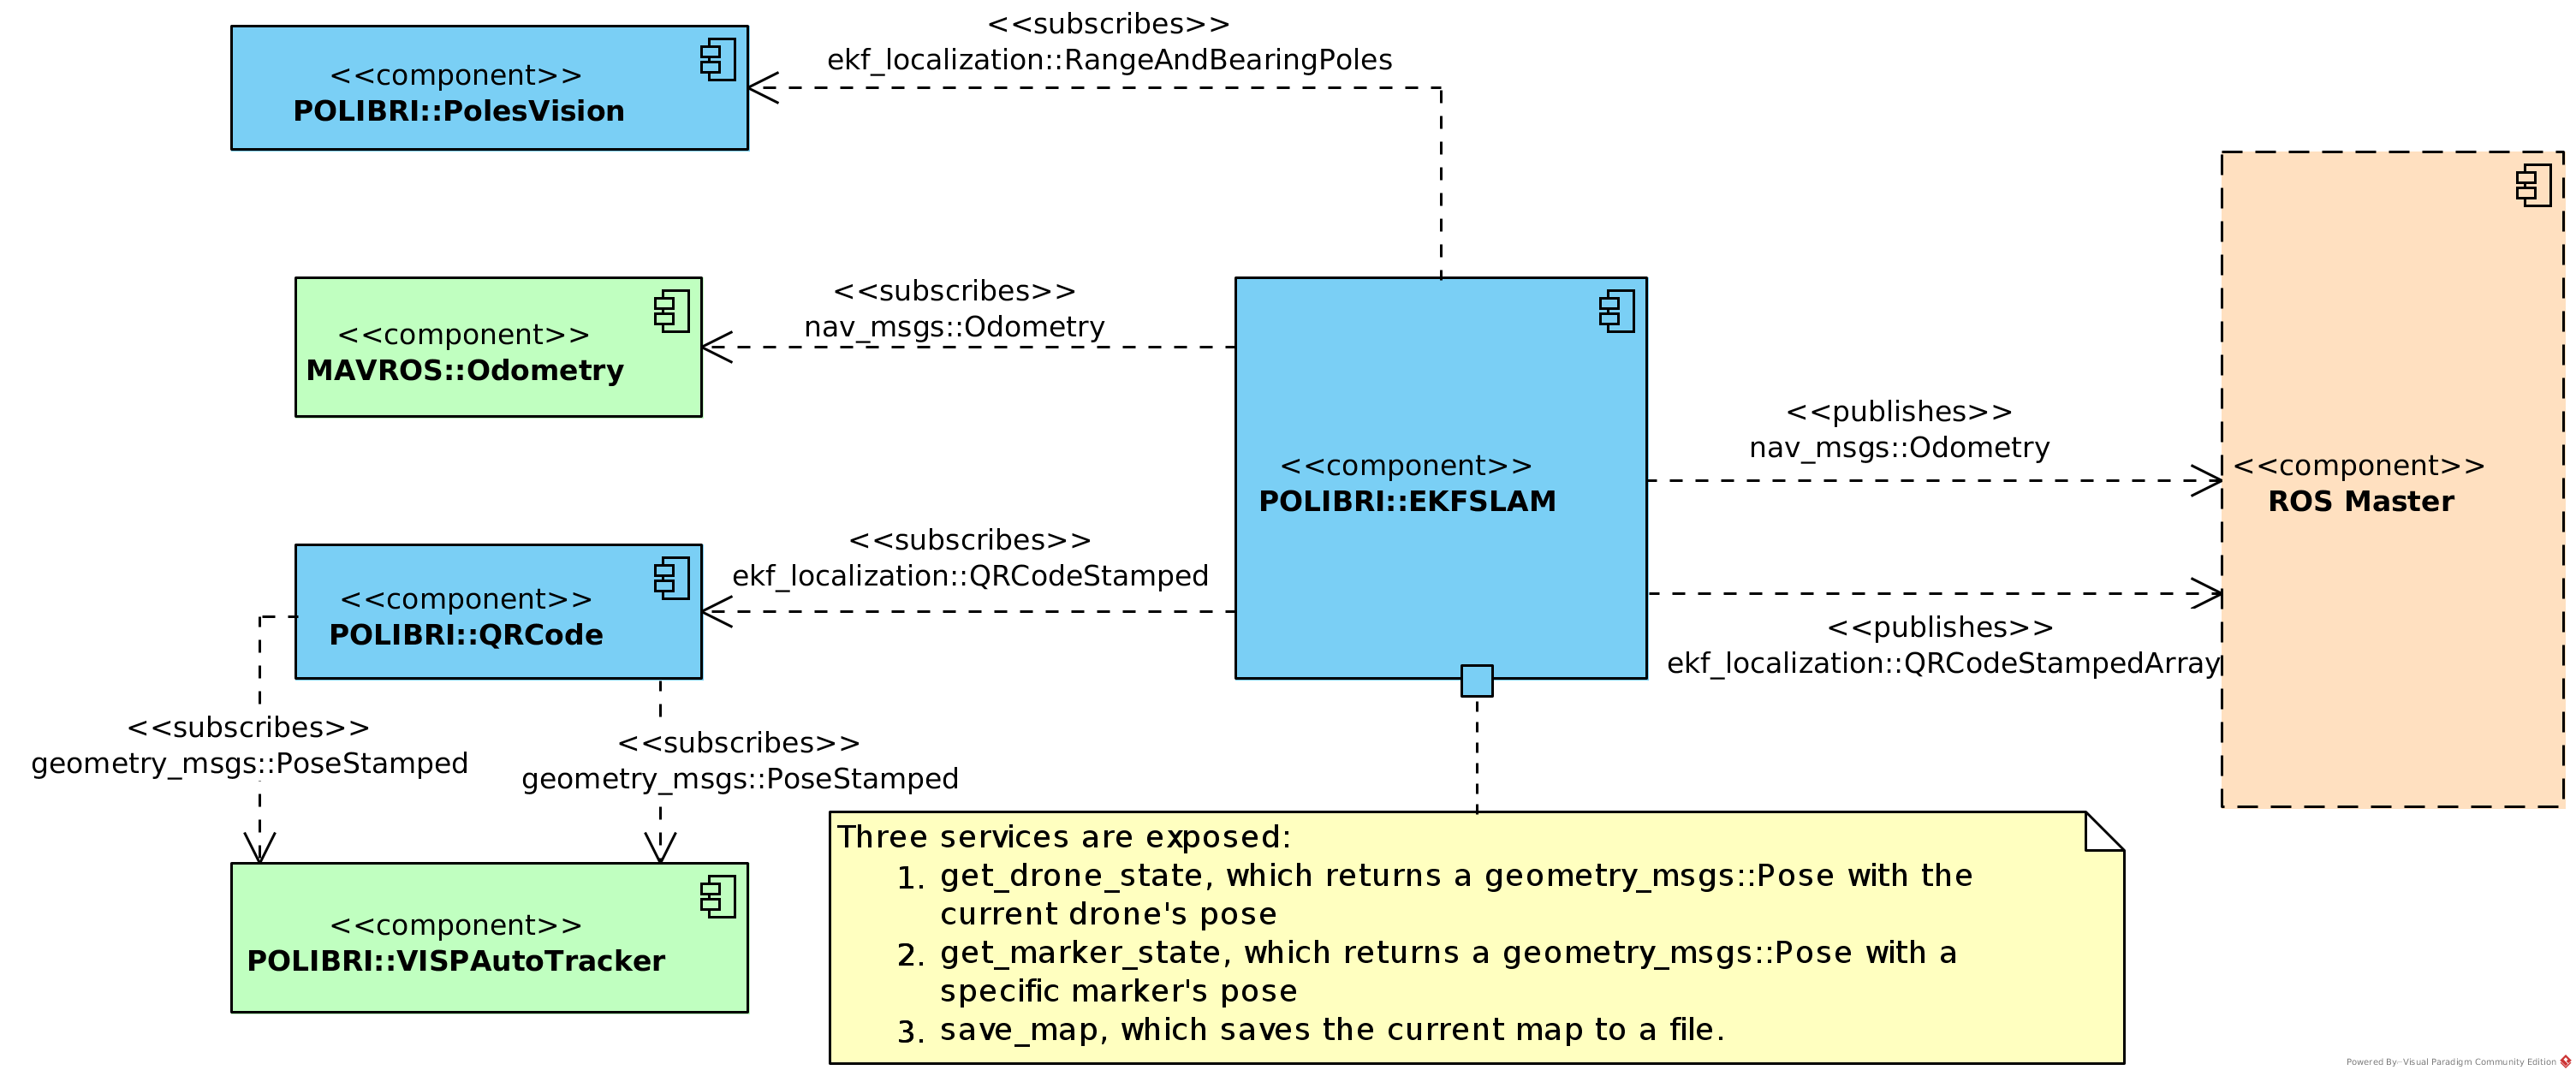
\includegraphics[width=\textwidth]{Images/fig9-components_diagram}
    \caption[Components diagram of the EKF Localization node]{Components diagram of the EKF Localization node. The \inlinesrc{EKFSLAM} class subscribes to different messages, between them the \inlinesrc{Odometry} messages are used as control variables, while the \inlinesrc{RangeAndBearingPole} and \inlinesrc{QRCodeStamped} messages are used every time the drone observes a pole or a marker. Moreover, \inlinesrc{EKFSLAM} class publishes two types of messages: \inlinesrc{Odometry} which provides the filtered localization and \inlinesrc{QRCodeStampedArray} which contains a list markers' poses.}
    \label{fig:chapter2:architecture:components}
\end{figure}

It is worth to mention that the messages of type \inlinesrc{QRCodeStamped} are provided by the \inlinesrc{QRCode} node which is internal to the \inlinesrc{ekf_localization} package. This node is needed because the \inlinesrc{visp_auto_tracker}, responsible of identifying the markers and publish their poses, publish these data as separate messages: the marker's id as a \inlinesrc{String} message and the pose as a \inlinesrc{PoseStamped} message. Due to this situation, the \inlinesrc{QRCode} node is responsible of match both data together and publish an \inlinesrc{QRCodeStamped} message which contains the marker's identifier and its pose.\\

\begin{figure}
    \centering
    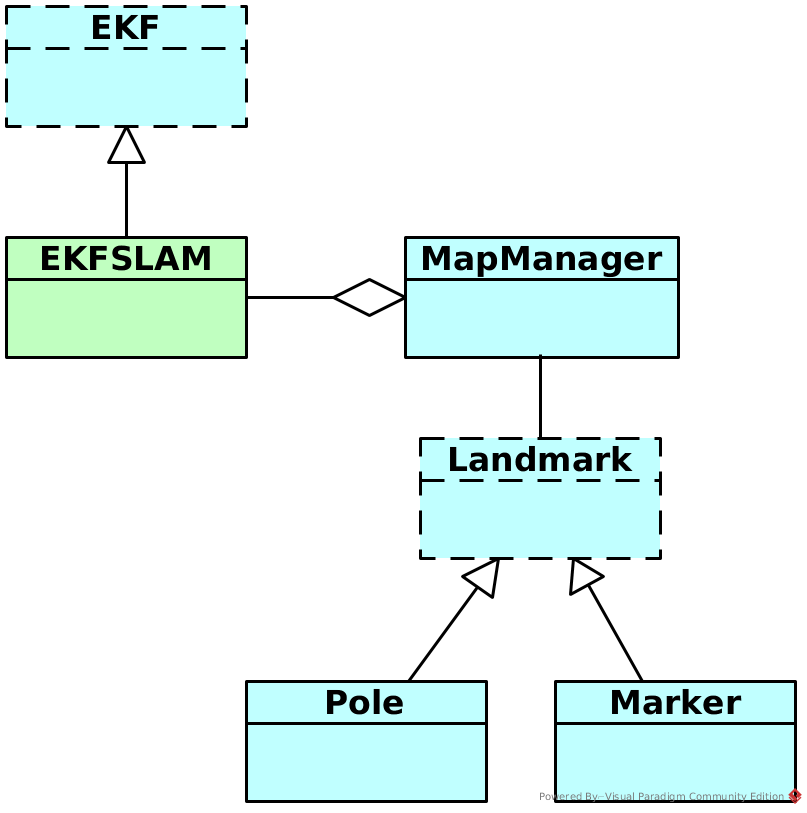
\includegraphics[width=0.5\textwidth]{Images/fig10-class_diagram}
    \caption[Class diagram of the EKFSLAM node]{Class diagram of the EKFSLAM node. The \inlinesrc{EKFSLAM} class is composed by a \inlinesrc{MapManager} instance, which is composed by a list of \inlinesrc{Landmarks}. The \inlinesrc{Landmark} class is abstract and its concrete classes are \inlinesrc{Pole} and \inlinesrc{Marker}.}
    \label{fig:chapter2:architecture:class}
\end{figure}

The main element of the EKF-SLAM node is the \inlinesrc{EKFSLAM} class which is responsible of keeping track of the state vector and execute the EKF-SLAM algorithm. This class inherit from an abstract class called \inlinesrc{EKF}, which is responsible of the implementation of the algorithm in a generic way, while the specifics for the current problem is contained in its child.\\

There are several components that interact within \inlinesrc{EKFSLAM} class, but probably the most interesting one is the \inlinesrc{MapManager} class. This class is responsible of maintaining an updated map of the environment with all the poles and markers, and to save and retrieve the map from a YAML file.\\

The \inlinesrc{MapManager} class contains a list of \inlinesrc{Landmark}s, and every time the state vector is updated in \inlinesrc{EKFSLAM} class, the \inlinesrc{MapManager} class updates the information about each \inlinesrc{Marker}. As mentioned before, the pose of each pole is known and needs no update. Furthermore, the \inlinesrc{Landmark} class is specialized in a \inlinesrc{Marker} class and a \inlinesrc{Pole} class, each of which is responsible of provide the observation model associated to it and the needed Jacobian matrices for the algorithm, hiding the implementation to the \inlinesrc{EKFSLAM} class.
\subsection{ROS nodes}
\label{subsec:chapter2:arch:nodes}
Regarding the ROS node that comprise the system, in Figure~\ref{fig:chapter2:architecture:nodes:all} all the ones that interact with the localization node are shown. The EKF-SLAM node is called \inlinesrc{/ekf_localization_node}, and as mentioned before, it interacts with \inlinesrc{/mavros} node, all the poles identification nodes (\inlinesrc{/poles_vision_#}), the \inlinesrc{/qr_code_node} which publishes the markers position with its identifier, and the \inlinesrc{/rtabmap} node that provides the Octomap messages. \\

As mentioned, the Figure~\ref{fig:chapter2:architecture:nodes:all} shows all the nodes (depicted as ellipses) with its interactions: a node publishes a message topic, and the topic is consumed by a node. This interaction is represented by the arrows, where an incoming arrow means that a node subscribes to the message topic, while an outgoing arrow means that the node publishes that message topic. Arrows go from a node to a topic or from a topic to a node, but do not go from node to node. Its reason lies on the fact that nodes interact between each other using a message passing interface as mention in Section~\ref{sec:chapter1:ros}. Furthermore, it is worth to mention that in Figure~\ref{fig:chapter2:architecture:nodes:all} a \inlinesrc{/gazebo} node is present. This node appears only on simulation and represents the simulated environment, that is why it publishes all the cameras and stereo cameras information.\\
\begin{figure}
    \centering
    \includegraphics[width=\textwidth]{Images/fig11-rosgraph_all}
    \caption[ROS graph of the system]{ROS graph of the system. Nodes are depicted as ellipses, while message topics are depicted as boxes. Each arrow means that a node publishes or subscribes to a specific message topic.}
    \label{fig:chapter2:architecture:nodes:all}
\end{figure}
Figure~\ref{fig:chapter2:architecture:nodes:ekf_node} shows the detail for the \inlinesrc{/ekf_localization_node} with all its subscriptions. It is worth to mention the \inlinesrc{/qr_code_node}, which subscribes to \inlinesrc{/visp_auto_tracker/code_message} and \inlinesrc{/visp_auto_tracker/object_position}, and publishes a \inlinesrc{/visp_auto_tracker/stamped_object_position}.
\begin{figure}[h]
    \centering
    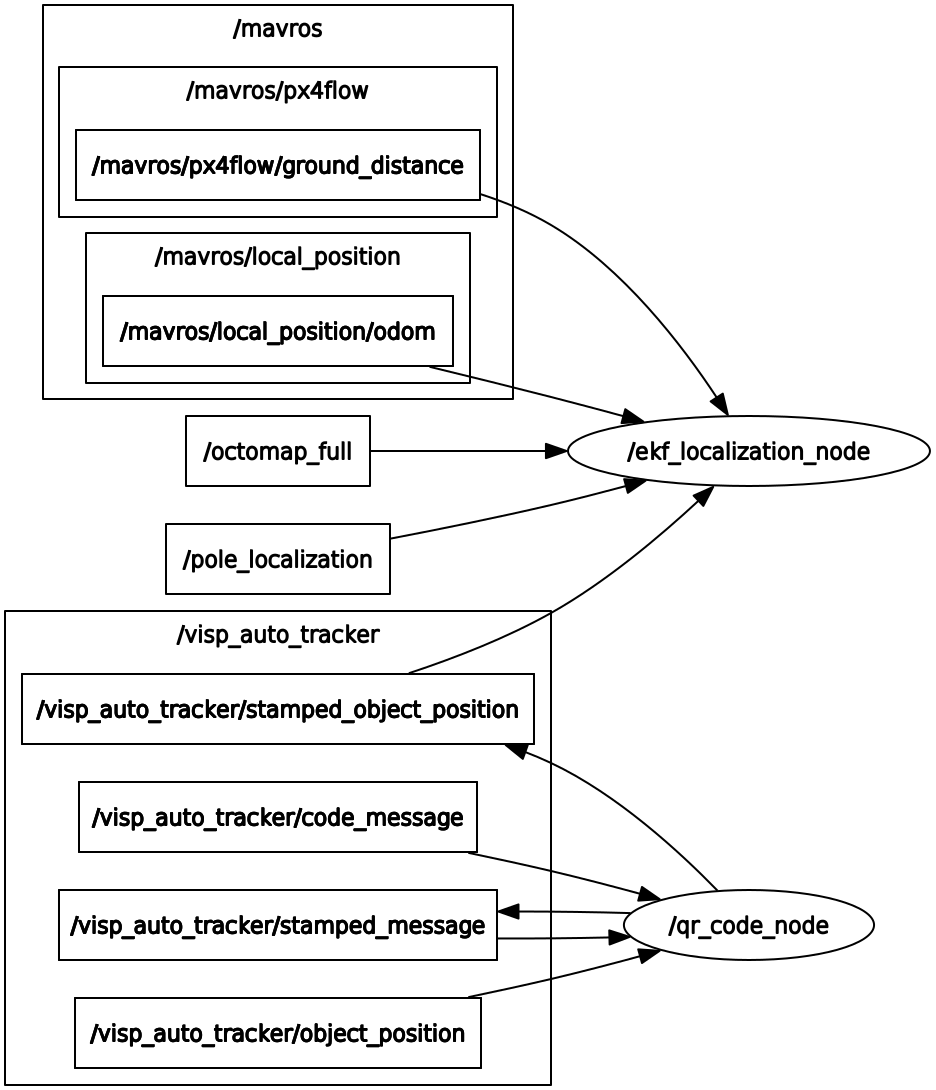
\includegraphics[width=0.8\textwidth]{Images/fig12-rosgraph_ekf_node}
    \caption[Detail of the EKF-SLAM node interactions]{Detail of the EKF-SLAM node interactions. Beside the \inlinesrc{/ekf_localization_node}, the \inlinesrc{/qr_node_code} can be seen. This node, is responsible of subscribing the \inlinesrc{/visp_auto_tracker} messages in order to, then, publish the identifier along with the pose of the marker that has been seen. On the other hand, the \inlinesrc{/ekf_localization_node} subscribes to the \inlinesrc{/mavros}, \inlinesrc{/octomap}, \inlinesrc{/pole_localization} and \inlinesrc{/visp_auto_tracker} messages.}
    \label{fig:chapter2:architecture:nodes:ekf_node}
\end{figure}





















	\chapter{Experimental Results}
\label{chapter3}

% Introduction where I should explain the purpose of the experiments.

\section{The Environment}
\label{sec:chapter3:environment}

\section{Simulated Experiments}
\label{sec:chapter3:simulation}

\subsection{Procedures}
\label{subsec:chapter3:simulation:procedures}

\subsection{Results}
\label{subsec:chapter3:simulation:results}

\section{Empirical Results ?}
\label{sec:chapter3:empirical}

\subsection{Procedures}
\label{subsec:chapter3:empirical:procedures}

\subsection{Results}
\label{subsec:chapter3:empirical:results}
	\chapter{Conclusions and Future Work}
\label{ch:chapter4}
In Chapter~\ref{ch:chapter2} the proposed implementation was presented and in Chapter~\ref{ch:chapter3}, experiments and their results were showed. This Chapter presents the conclusions related to the performed experiments, and some thoughts about the proposed implementation.\\

Moreover, future lines of research are proposed for localization and mapping in the context of the Leonardo Drone Contest environment.

\section{Conclusions}
The EKF-SLAM algorithm is a proved and extensively used algorithm for localization and mapping problems in robotics. The \ac{KF} introduced in 1960, later refined for non-linear systems and introduced in \cite{ekf-slam-smith} for localization and mapping problems, is implemented by this work. The proposed implementation was developed in the context of the Leonardo Drone Contest, which has specific characteristics.\\

Several experiments were conducted with the aim of identifying specific characteristics and implementation details that are important for the objective of the algorithm. In this sense, and as explained in Chapter~\ref{ch:chapter3}, four set of experiments were conducted, each of them with a specific objective. From these experiments, some conclusions can be extracted.\\

The first two sets of experiments shed some light about the importance of different types of landmarks, in this particular case, poles and markers. These experiments showed the importance of poles in the correction of X, Y and Z position and the orientation of the drone, and the importance of markers in the localization process. Moreover, the correction of drone's pose is important also for the prediction of the markers' poses as it can be seen in Table~\ref{tab:chapter3:simulated:experiments:b:distance}. The average Euclidean distance of the four markers is 0.134, which is good enough for the contest but also perfectible. The same can be observed in the case of the orientation, which in the worst case is 3\textdegree.\\

The third experiment showed that the height estimation can be corrected using a combination of Octomap and range sensor. As mentioned in Section~\ref{subsubsec:chapter3:simulation:c:results} a key component for the height estimation is the completeness and correctness of the Octomap. This experiment showed that when the Octomap and the sensor range produce good measurements, the height estimation follows the ground truth. However, the experiment could be defined as not conclusive since the amount of time with Octomap measurements is low: only 70 seconds out of 363.\\

Finally, the last set of experiments showed the importance of the \ac{NEES} test for the consistency of the filter. As can be appreciated in Figure~\ref{fig:chapter3:simulation:d:no-nees-test}, when no \ac{NEES} test is used, the pose correction is not good enough to be used in any environment. It can be concluded that \ac{NEES} is needed to filter out invalid measurements. However, a value of $\chi^2$ needs to be found in order to achieve better performance. As showed in Figure~\ref{fig:chapter3:simulation:d:nees-10-discarded-markers}, lower confidence of valid measurements makes the filter discard truly bad measurements, but on the other hand it can discard measurements that can be useful to correct the drone's pose. The $\chi^2$ value should be set for every type of landmark, thus it becomes a new parameter to be tuned in the filter.\\

It can be concluded that the current implementation works well in the current environment and in the context of the used \ac{ROS} bags. However, a fine tuning is needed in order to improve its performance in simulation. The observation noise covariance matrices were barely tuned, and the $\chi^2$ values used were the most common ones (confidence of 95\%).\\

As mentioned before, EKF-SLAM is a proved algorithm and works with a decent performance in the current environment. The proposed implementation sets the bases for future developments and improvements, and can be used as baseline for comparison with more complex or novel algorithms. Moreover, the proposed implementation can be extended in order to be applied in other indoor or GNSS-denied environments with minimum modifications. Its architecture was thought to be slightly coupled and highly extensible in the sense that new landmarks and observations types can be added in an easy way.

\section{Future Work}
As stated in Chapter~\ref{ch:chapter0:intro}, the current implementation could not be deployed and tested in the real drone, hence it would be an important step to evaluate it. The real drone experimentation should be done considering both poles and markers for the localization. Moreover, the performance while mapping the environment should be evaluated, as well as the height correction.\\

As already stated, the current implementation is perfectible and can be improved in different ways. Fine tuning of the algorithm's parameters to improve its performance is needed. Another improvement could be a camera self calibration procedure to improve the Z position estimation using poles and markers. Also, extensive experimentation with Octomap and range sensor for height update is needed.\\

Additionally, it could be possible to compare the current algorithm with other algorithms like Error-State EKF-SLAM, or \ac{UKF} SLAM, and evaluate their performance with the current implementation as baseline.



	% ************************************************************
	% Backmatter
	%*************************************************************
	\cleardoublepage%********************************************************************
% Bibliography
%*******************************************************
% work-around to have small caps also here in the headline
\manualmark
\markboth{\spacedlowsmallcaps{\bibname}}{\spacedlowsmallcaps{\bibname}}
%\phantomsection 
\refstepcounter{dummy} 
% to have the bib a bit from the rest in the toc
\addtocontents{toc}{\protect\vspace{\beforebibskip}}
\addcontentsline{toc}{chapter}{\tocEntry{\bibname}}
\label{app:bibliography} 
\printbibliography
	\appendix
%	\cleardoublepage\part{Appendix}
	\chapter{Source Code}
\label{appendix:a}
    \chapter{User Manual}
\label{appendix:b}

\end{document}
% ****************************************************************